\documentclass[11pt]{article}

\usepackage[utf8]{inputenc}
\usepackage{graphicx}
\usepackage{geometry}
\usepackage{xcolor}
\usepackage{titlesec}
\usepackage{fancyhdr}
\usepackage{tocloft}
\usepackage{float}

\usepackage[colorlinks=true, linkcolor=black, urlcolor=black, citecolor=black]{hyperref}

\geometry{margin=2.5cm}


\definecolor{myblue}{HTML}{2C56C9}
\definecolor{myline}{HTML}{253555}

\titleformat{\section}
{\color{myblue}\normalfont\Large\bfseries}
{\thesection}{1em}{}

\fancypagestyle{normal}{
    \fancyhf{}
    \fancyhead[L]{\textcolor{myblue}{Corsi di Studi in Informatica}}
    \fancyhead[R]{\textcolor{myblue}{00BD39}}
    \fancyfoot[L]{\textcolor{myblue}{UninaFoodLab}}
    \fancyfoot[C]{\thepage}
    \fancyfoot[R]{\textcolor{myblue}{2025/2026}}
    \renewcommand{\headrulewidth}{0.4pt}
    \renewcommand{\footrulewidth}{0.4pt}
    \renewcommand{\headrule}{\color{myline}\hrule height 0.4pt \vspace{3pt}}
    \renewcommand{\footrule}{\color{myline}\hrule height 0.4pt \vspace{3pt}}
}

\fancypagestyle{firstpage}{
    \fancyhf{}
    \fancyfoot[L]{\textcolor{myblue}{UninaFoodLab}}
    \fancyfoot[C]{\thepage}
    \fancyfoot[R]{\textcolor{myblue}{2025/2026}}
    \renewcommand{\headrulewidth}{0pt}
    \renewcommand{\footrulewidth}{0.4pt}
    \renewcommand{\footrule}{\color{myline}\hrule height 0.4pt \vspace{3pt}}
}



\renewcommand{\contentsname}{Indice}
\renewcommand{\cftsecfont}{\color{myblue}\bfseries}

\begin{document}



\thispagestyle{firstpage}


\begin{center}
    
\includegraphics[width=0.3\textwidth]{latex/immagini/uni_logo.png} 
    \vspace{0.5cm}

    {\large \textbf{Corso di Laurea in Informatica - Università degli Studi di Napoli Federico II}}\\
    {\large \textbf{A.A. 2025/2026}}\\[1cm]
    \vspace{1cm}

    {\Huge \color{myblue} \textbf{UninaFoodLab}}\\[2cm]

    \begin{flushleft}
    \centering
    {\large
    \textbf{Calone Francesco N86005555}\\
    \vspace{0.2cm}
    \textbf{D'Angelo Mario N86005477}\\
    }
    
    \vspace{0.2cm}
    {\small Codice gruppo: \textbf{OOBD39}}\\
    \vspace{0.8cm} 

    {\small Insegnamento di Programmazione Object-Oriented}
    \end{flushleft}
\end{center}


\newpage

\pagestyle{normal}

\tableofcontents
\thispagestyle{normal}

\section{Introduzione}

Il progetto UninaFoodLab nasce con l'obiettivo di offrire una soluzione software moderna e intuitiva per la gestione di corsi culinari. La piattaforma è stata sviluppata seguendo le best practice adottando tecnologie consolidate come JavaFX per la realizzazione dell'interfaccia grafica e Maven per la gestione delle dipendenze e dei processi di build.
Il progetto è stato concepito per essere facilmente estendibile e manutenibile, grazie a una chiara separazione dei livelli logici.
La documentazione che segue illustra le scelte progettuali, le tecnologie utilizzate e le principali funzionalità implementate, con l'intento di fornire una panoramica completa e professionale del sistema sviluppato.
\subsection{Obiettivi del Progetto}
Il progetto UninaFoodLab si propone di:
\begin{itemize}
    \item Fornire una piattaforma intuitiva per la gestione di corsi culinari
    \item Semplificare la registrazione e la gestione degli utenti e per gli chef
    \item Facilitare la creazione e la gestione dei corsi, inclusa la pianificazione delle lezioni e la gestione delle ricette
    \item Semplificare la gestione delle prenotazioni e dei pagamenti per i corsi
\end{itemize}

\section{progettazione concettuale}
\subsection{Introduzione}
Il modello concettuale rappresenta la struttura logica del database, definendo le entità, gli attributi e le relazioni tra di esse. In questa fase, si è proceduto a identificare le principali entità del sistema e a stabilire le relazioni che le collegano, garantendo così una visione chiara e coerente delle informazioni da gestire.
\subsection{UML non ristrutturato}
\begin{figure}[H]
    \noindent\makebox[\linewidth]{%
        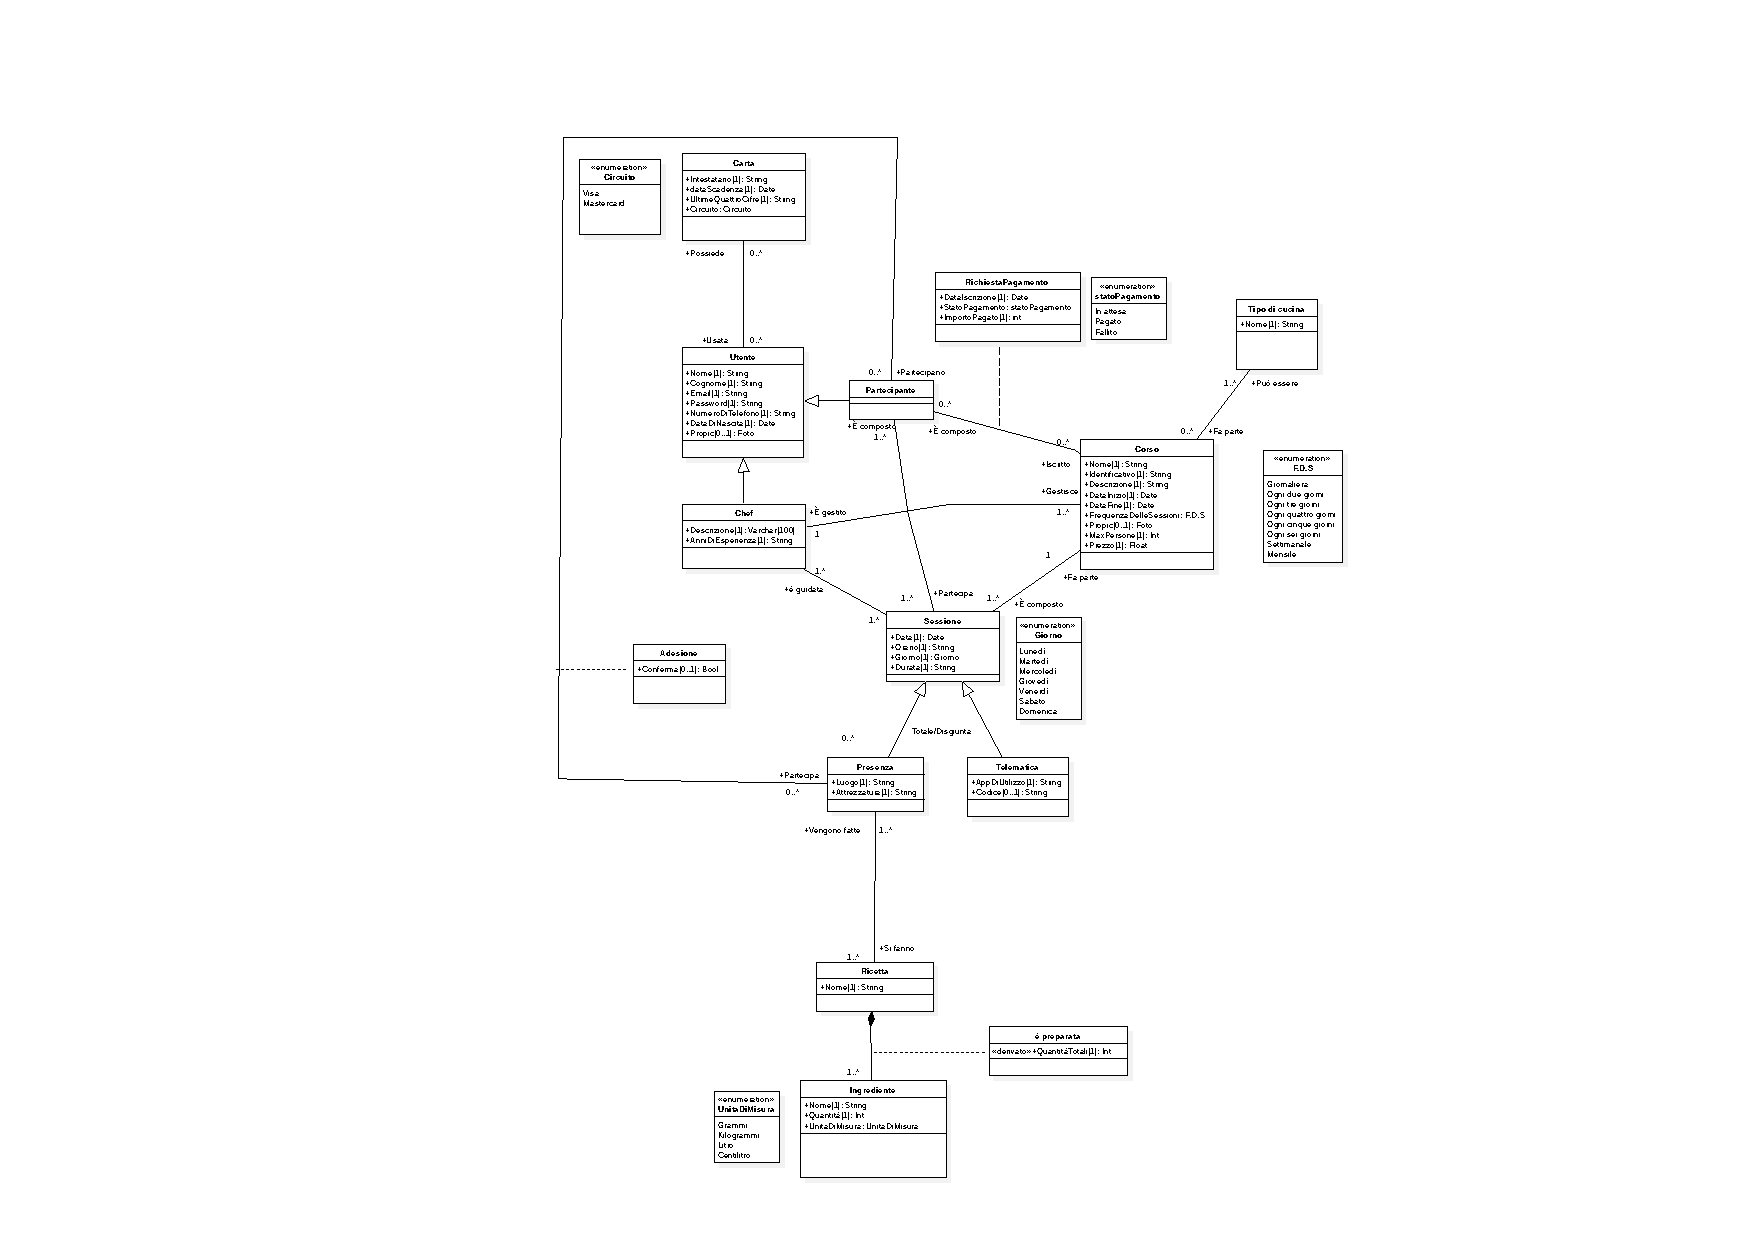
\includegraphics[height=0.9\textheight,width=2\textwidth]{latex/immagini/uml_non_ristrutturato.pdf}
    }
    \caption{Diagramma UML del sistema}
\end{figure}
\subsubsection{Entità principali}
Le entità principali identificate nel sistema sono:
\begin{itemize}
    \item \textbf{Utente}: L’utente rappresenta il soggetto fruitore del sistema, che può iscriversi ai corsi e partecipare alle sessioni. I principali attributi includono nome, cognome, email, password, telefono, data di nascita e una foto di profilo. Ogni utente può essere associato a una o più carte di pagamento e può diventare partecipante a diversi corsi.
    \item \textbf{Chef}: Lo chef è un utente con il ruolo specifico di organizzare corsi. Ogni chef dispone di una descrizione e di un numero di anni di esperienza. Un chef può gestire più corsi, ma ogni corso è gestito da un solo chef.
    \item \textbf{Corso}: Il corso è l'entità centrale del sistema e rappresenta una proposta didattica su un tema gastronomico specifico. Contiene attributi quali nome, descrizione, identificativo, data di inizio/fine, frequenza delle sessioni, prezzo, immagine di copertina e tipo di cucina (modellato come enumerazione). Ogni corso è composto da più sessioni e prevede una relazione molti-a-molti con i partecipanti.
    \item \textbf{Sessione}: Ogni corso è articolato in una o più sessioni, ciascuna delle quali ha una data, un orario, un insieme di giorni della settimana in cui si svolge, e una durata. Le sessioni sono specializzate in due sottotipi mutuamente esclusivi:
    \begin{itemize}
        \item \textbf{Presenza}: Con attributi come luogo e attrezzature richieste.
        \item \textbf{Telematica}: Con attributi relativi all'app utilizzata e al codice di accesso.
    \end{itemize}
    \item \textbf{Partecipante e Adesione}: La partecipazione ai corsi è modellata tramite l’entità Partecipante, che collega utenti e corsi. La partecipazione a sessioni pratiche richiede un’adesione esplicita, rappresentata dall'entità Adesione, che contiene un attributo booleano di conferma.
    \item \textbf{Ricetta e Ingredientemento}: Ogni sessione pratica può includere la preparazione di una o più ricette. Ogni ricetta è composta da uno o più ingredienti, ciascuno dei quali ha un nome, una quantità e un'unità di misura (enumerata). La relazione tra Ricetta e Ingrediente è associativa e include l'attributo QuantitàTotale, utile per calcolare la quantità necessaria in base alle adesioni.
    \item \textbf{Carta e RichiestaPagamento}: Gli utenti possono associare al proprio profilo una o più carte di pagamento, appartenenti a un circuito specificato tramite enumerazione (Visa, Mastercard). Le richieste di pagamento sono entità separate, con data, stato (in attesa, pagato, fallito) e importo.
\end{itemize}
\subsubsection{Gerarchie e generalizzazioni}
Nel modello concettuale, sono state identificate le seguenti gerarchie e generalizzazioni:
\begin{itemize}
    \item \textbf{Sessione}: Le sessioni sono suddivise in due sottotipi: \textit{Presenza} e \textit{Telematica}. Questa specializzazione consente di gestire le specificità di ciascun tipo di sessione, come il luogo e le attrezzature per le sessioni in presenza, e l'app utilizzata e il codice di accesso per quelle telematiche.
    \item \textbf{Utente}: L'entità Utente può essere specializzata in due sottotipi: \textit{Partecipante} e \textit{Chef}. Questa distinzione permette di gestire le diverse funzionalità e attributi associati a ciascun ruolo nel sistema.
\end{itemize}
Entrambe le specializzazioni sono totali e disgiunte, di conseguenza ogni istanza di Sessione sia esclusivamente di uno dei due tipi e che ogni Utente sia o un Partecipante o uno Chef, ma non entrambi contemporaneamente.
\subsubsection{Relazioni tra le entità}
Le relazioni tra le entità sono state definite come segue:
\begin{itemize}
    \item \textbf{Utente - Partecipante}: Un utente può essere un partecipante a più corsi, e ogni corso può avere più partecipanti. Questa relazione è molti-a-molti.
    \item \textbf{Chef - Corso}: Ogni chef può gestire più corsi, ma ogni corso è associato a un solo chef. Questa relazione è uno-a-molti.
    \item \textbf{Corso - Sessione}: Un corso può avere più sessioni, ma ogni sessione appartiene a un solo corso. Questa relazione è uno-a-molti.
    \item \textbf{Sessione - Partecipante}: Ogni partecipante può aderire a più sessioni pratiche, e ogni sessione può avere più partecipanti. Questa relazione è molti-a-molti, mediata dall'entità Adesione.
    \item \textbf{Corso - Ricetta}: Ogni corso può includere più ricette, e ogni ricetta può essere associata a più corsi. Questa relazione è molti-a-molti.
    \item \textbf{Ricetta - Ingrediente}: Ogni ricetta può includere più ingredienti, e ogni ingrediente può essere utilizzato in più ricette. Questa relazione è molti-a-molti, mediata dall'attributo QuantitàTotale.
    \item \textbf{Utente - Carta}: Un utente può avere più carte di pagamento associate al proprio profilo. Questa relazione è uno-a-molti.
    \item \textbf{Ricetta - Ingrediente}: Ogni ricetta può essere associata a più ingredienti, e ogni ingrediente può essere utilizzato in più ricette. Questa relazione è una composizione, mediata dall'attributo QuantitàTotale.
\end{itemize}
\subsubsection{Motivazione delle scelte progettuali}
Le scelte progettuali sono state guidate dalla necessità di garantire una rappresentazione chiara e coerente delle informazioni, facilitando la gestione dei corsi, delle sessioni e delle partecipazioni. La specializzazione delle sessioni in Presenza e Telematica consente di gestire le specificità di ciascun tipo di sessione, mentre la distinzione tra Partecipante e Chef permette di differenziare i ruoli degli utenti nel sistema. Inoltre, l'uso di relazioni molti-a-molti per gestire le adesioni alle sessioni pratiche e le associazioni tra ricette e ingredienti garantisce flessibilità e scalabilità nel modello.



\section{Architettura del Progetto}

L'architettura del progetto UninaFoodLab è stata progettata per garantire una chiara separazione dei compiti e una facile manutenibilità. La struttura delle directory riflette i principali livelli logici dell'applicazione, secondo il pattern MVC e le best practice di progettazione.

Le principali suddivisioni sono:
\begin{itemize}
    \item \textbf{Boundary}: contiene le classi responsabili dell'interfaccia grafica e dell'interazione con l'utente, realizzate tramite JavaFX e FXML.
    \item \textbf{Controller}: gestisce la logica applicativa e il flusso degli eventi tra la GUI e i dati.
    \item \textbf{Entity}: suddivisa ulteriormente in \textit{DAO} (Data Access Object) e \textit{DTO} (Data Transfer Object). I DAO si occupano della persistenza e dell'accesso ai dati, mentre i DTO rappresentano le strutture dati scambiate tra i vari livelli.
    \item \textbf{JDBC}: contiene le classi e le utility per la connessione e la gestione del database PostgreSQL.
    \item \textbf{Utils}: raccoglie le classi di supporto e gli strumenti riutilizzabili all'interno del progetto.
\end{itemize}
Questa organizzazione favorisce la modularità e la scalabilità del sistema, permettendo di isolare le responsabilità e facilitare l'estensione futura. Ogni componente interagisce con gli altri tramite interfacce ben definite, riducendo le dipendenze e migliorando la qualità del codice.

La scelta di suddividere le entity in DAO e DTO consente di gestire in modo efficiente sia la persistenza che il trasferimento dei dati, mentre la presenza di una directory dedicata alle utility semplifica la gestione delle funzionalità trasversali.

\subsection{Struttura delle Directory}
La struttura delle directory del progetto è organizzata come segue:
\begin{itemize}
    \item \textbf{src/main/java}: contiene il codice sorgente dell'applicazione.
    \item \textbf{src/main/resources}: contiene le risorse dell'applicazione, come file FXML e immagini.
    \item \textbf{src/test/java}: contiene i test automatizzati.
\end{itemize}


\section{Definizioni SQL}

\subsection{Introduzione}

In questo capitolo viene presentata l'implementazione pratica del database UninaFoodLab attraverso la definizione completa del codice SQL sviluppato in PostgreSQL. La sezione fornisce una panoramica dettagliata di tutti gli elementi che compongono il database, dalla creazione delle tabelle all'implementazione delle funzioni.


\subsection{Definizione degli enumerati}

Gli enumerati sono tipi di dato definiti dall’utente che permettono di vincolare il valore di un attributo a un insieme finito di possibilità predefinite. Nel database UninaFoodLab vengono utilizzati per rappresentare domini chiusi come circuiti di carte, stati di pagamento, frequenza delle sessioni, giorni della settimana e unità di misura degli ingredienti. Questo garantisce coerenza e integrità dei dati, semplificando la gestione delle regole applicative.

\noindent\rule{\textwidth}{0.4pt}
\begin{lstlisting}[language=SQL, style=sqlstyle, literate={à}{{\`a}}1 {è}{{\`e}}1 {é}{{\'e}}1 {ì}{{\`i}}1 {ò}{{\`o}}1 {ù}{{\`u}}1]
CREATE TYPE Circuito AS ENUM ('Visa', 'Mastercard');

CREATE TYPE StatoPagamento AS ENUM ('In attesa', 'Pagato', 'Fallito');

CREATE TYPE FDS AS ENUM (
  'Giornaliera',
  'Ogni due giorni',
  'Ogni tre giorni',
  'Ogni quattro giorni',
  'Ogni cinque giorni',
  'Ogni sei giorni',
  'Settimanale',
  'Mensile'
);

CREATE TYPE Giorno AS ENUM (
  'Lunedì',
  'Martedì',
  'Mercoledì',
  'Giovedì',
  'Venerdì',
  'Sabato',
  'Domenica'
);

CREATE TYPE UnitaDiMisura AS ENUM ('Grammi', 'Kilogrammi', 'Litro', 'Centilitro');
\end{lstlisting}
\noindent\rule{\textwidth}{0.4pt}

\subsection{Definizione delle Tabelle}


\subsubsection{Tabella Partecipante}

La tabella \texttt{Partecipante} rappresenta gli utenti che si iscrivono e partecipano ai corsi di cucina. Ogni partecipante ha un identificativo univoco generato automaticamente e deve fornire informazioni personali essenziali per la registrazione.

\noindent\rule{\textwidth}{0.4pt}
\begin{lstlisting}[language=SQL, style=sqlstyle]
CREATE TABLE Partecipante (
    IdPartecipante INT GENERATED ALWAYS AS IDENTITY PRIMARY KEY,
    Nome VARCHAR(50) NOT NULL,
    Cognome VARCHAR(50) NOT NULL,
    Email VARCHAR(100) UNIQUE NOT NULL,
    Password VARCHAR(100) NOT NULL,
    DataDiNascita DATE NOT NULL,
    Propic TEXT
);
\end{lstlisting}
\noindent\rule{\textwidth}{0.4pt}

\textbf{Scelte progettuali:}
\begin{itemize}
    \item \textbf{IdPartecipante}: Chiave primaria auto-incrementale utilizzando \texttt{GENERATED ALWAYS AS IDENTITY} per garantire unicità automatica
    \item \textbf{Email}: Constraint \texttt{UNIQUE} per evitare registrazioni duplicate
    \item \textbf{Password}: Campo di lunghezza fissa per supportare hash di password sicure
    \item \textbf{Propic}: Campo \texttt{TEXT} per supportare URL di immagini o dati base64
\end{itemize}

\subsubsection{Tabella Carta}

La tabella \texttt{Carta} memorizza le carte di pagamento associate agli utenti. Ogni carta ha un identificativo univoco, intestatario, data di scadenza, ultime quattro cifre e circuito di appartenenza.

\noindent\rule{\textwidth}{0.4pt}
\begin{lstlisting}[language=SQL, style=sqlstyle]
CREATE TABLE Carta (
    IdCarta INT GENERATED ALWAYS AS IDENTITY PRIMARY KEY,
    Intestatario VARCHAR(100) NOT NULL,
    DataScadenza DATE NOT NULL,
    UltimeQuattroCifre CHAR(4) NOT NULL,
    Circuito VARCHAR(50) NOT NULL
);
\end{lstlisting}
\noindent\rule{\textwidth}{0.4pt}

\textbf{Scelte progettuali:}
\begin{itemize}
    \item \textbf{IdCarta}: Chiave primaria auto-incrementale
    \item \textbf{Intestatario, DataScadenza, UltimeQuattroCifre, Circuito}: Attributi essenziali per identificare una carta
    \item \textbf{Circuito}: Vincolato tramite tipo enumerato per coerenza
\end{itemize}

\subsubsection{Tabella Possiede}

La tabella \texttt{Possiede} rappresenta la relazione molti-a-molti tra partecipanti e carte, indicando quali carte sono possedute da ciascun partecipante.

\noindent\rule{\textwidth}{0.4pt}
\begin{lstlisting}[language=SQL, style=sqlstyle]
CREATE TABLE Possiede (
    IdPartecipante INT,
    IdCarta INT,
    PRIMARY KEY (IdPartecipante, IdCarta),
    FOREIGN KEY (IdPartecipante) REFERENCES Partecipante(IdPartecipante),
    FOREIGN KEY (IdCarta) REFERENCES Carta(IdCarta) on delete cascade 
);
\end{lstlisting}
\noindent\rule{\textwidth}{0.4pt}

\textbf{Scelte progettuali:}
\begin{itemize}
    \item \textbf{Chiave primaria composta}: (IdPartecipante, IdCarta) per garantire unicità della relazione
    \item \textbf{Vincoli di integrità}: Foreign key verso \texttt{Partecipante} e \texttt{Carta}
    \item \textbf{Cascata}: Eliminazione a cascata delle carte
\end{itemize}

\subsubsection{Tabella Corso}

La tabella \texttt{Corso} rappresenta i corsi di cucina offerti, con informazioni su nome, descrizione, periodo, frequenza, prezzo, chef responsabile e limiti di partecipazione.

\noindent\rule{\textwidth}{0.4pt}
\begin{lstlisting}[language=SQL, style=sqlstyle]
CREATE TABLE Corso (
    IdCorso INT GENERATED ALWAYS AS IDENTITY PRIMARY KEY,
    Nome VARCHAR(100) NOT NULL,
    Descrizione VARCHAR(60) NOT NULL,
    DataInizio DATE NOT NULL,
    DataFine DATE NOT NULL,
    FrequenzaDelleSessioni VARCHAR(100) NOT NULL,
    Propic TEXT,
    MaxPersone INT CHECK (MaxPersone > 0),
    Prezzo DECIMAL(10, 2) CHECK (Prezzo >= 0),
    IdChef INT NOT NULL,
    FOREIGN KEY (IdChef) REFERENCES Chef(IdChef)
);
\end{lstlisting}
\noindent\rule{\textwidth}{0.4pt}

\textbf{Scelte progettuali:}
\begin{itemize}
    \item \textbf{IdCorso}: Chiave primaria auto-incrementale
    \item \textbf{MaxPersone, Prezzo}: Vincoli di validità sui valori
    \item \textbf{IdChef}: Foreign key verso chef responsabile
    \item \textbf{FrequenzaDelleSessioni}: Vincolata tramite tipo enumerato
\end{itemize}

\subsubsection{Tabella RichiestaPagamento}

La tabella \texttt{RichiestaPagamento} registra le richieste di pagamento per i corsi, associando ogni richiesta a un partecipante e a un corso specifico, con informazioni su importo, stato e data.

\noindent\rule{\textwidth}{0.4pt}
\begin{lstlisting}[language=SQL, style=sqlstyle]
CREATE TABLE RichiestaPagamento (
    DataRichiesta TIMESTAMP NOT NULL,
    StatoPagamento VARCHAR(50) NOT NULL,
    ImportoPagato DECIMAL(10, 2) CHECK (ImportoPagato >= 0),
    IdCorso INT,
    IdPartecipante INT,
    PRIMARY KEY (DataRichiesta, IdCorso, IdPartecipante),
    FOREIGN KEY (IdCorso) REFERENCES Corso(IdCorso),
    FOREIGN KEY (IdPartecipante) REFERENCES Partecipante(IdPartecipante)
);
\end{lstlisting}
\noindent\rule{\textwidth}{0.4pt}

\textbf{Scelte progettuali:}
\begin{itemize}
    \item \textbf{Chiave primaria composta}: (DataRichiesta, IdCorso, IdPartecipante)
    \item \textbf{ImportoPagato}: Vincolo di non negatività
    \item \textbf{StatoPagamento}: Vincolato tramite tipo enumerato
    \item \textbf{Foreign key}: Collegamento a corso e partecipante
\end{itemize}

\subsubsection{Tabella TipoDiCucina}

La tabella \texttt{TipoDiCucina} elenca le tipologie di cucina disponibili, ciascuna con un identificativo univoco e un nome.

\noindent\rule{\textwidth}{0.4pt}
\begin{lstlisting}[language=SQL, style=sqlstyle]
CREATE TABLE TipoDiCucina (
    IDTipoCucina INT GENERATED ALWAYS AS IDENTITY PRIMARY KEY,
    Nome VARCHAR(50) NOT NULL UNIQUE
);
\end{lstlisting}
\noindent\rule{\textwidth}{0.4pt}

\textbf{Scelte progettuali:}
\begin{itemize}
    \item \textbf{IDTipoCucina}: Chiave primaria auto-incrementale
    \item \textbf{Nome}: Unicità per evitare duplicati
\end{itemize}

\subsubsection{Tabella TipoDiCucina\_Corso}

La tabella \texttt{TipoDiCucina\_Corso} rappresenta l'associazione tra corsi e tipologie di cucina, permettendo di collegare più tipi di cucina a ciascun corso (fino a un massimo di due).

\noindent\rule{\textwidth}{0.4pt}
\begin{lstlisting}[language=SQL, style=sqlstyle]
CREATE TABLE TipoDiCucina_Corso (
    IDTipoCucina INT,
    IDCorso INT,
    PRIMARY KEY (IDTipoCucina, IDCorso),
    FOREIGN KEY (IDTipoCucina) REFERENCES TipoDiCucina(IDTipoCucina),
    FOREIGN KEY (IDCorso) REFERENCES Corso(IdCorso)
);
\end{lstlisting}
\noindent\rule{\textwidth}{0.4pt}

\textbf{Scelte progettuali:}
\begin{itemize}
    \item \textbf{Chiave primaria composta}: (IDTipoCucina, IDCorso)
    \item \textbf{Foreign key}: Collegamento a tipo di cucina e corso
    \item \textbf{Vincolo applicativo}: Massimo due tipi di cucina per corso (gestito da trigger)
\end{itemize}

\subsubsection{Tabella Chef}

La tabella \texttt{Chef} contiene le informazioni sugli chef che tengono i corsi. Oltre ai dati anagrafici, include una descrizione e gli anni di esperienza.

\noindent\rule{\textwidth}{0.4pt}
\begin{lstlisting}[language=SQL, style=sqlstyle]
CREATE TABLE Chef (
    IdChef INT GENERATED ALWAYS AS IDENTITY PRIMARY KEY,
    Nome VARCHAR(50) NOT NULL,
    Cognome VARCHAR(50) NOT NULL,
    Email VARCHAR(100) UNIQUE NOT NULL,
    Password VARCHAR(100) NOT NULL,
    DataDiNascita DATE NOT NULL,
    Descrizione VARCHAR(60),
    Propic TEXT,
    AnniDiEsperienza INT CHECK (AnniDiEsperienza >= 0)
);
\end{lstlisting}
\noindent\rule{\textwidth}{0.4pt}

\textbf{Scelte progettuali:}
\begin{itemize}
    \item \textbf{IdChef}: Chiave primaria auto-incrementale
    \item \textbf{Email}: Unicità per evitare duplicati
    \item \textbf{AnniDiEsperienza}: Vincolo di non negatività
    \item \textbf{Propic}: Supporto per immagine profilo
\end{itemize}

\subsubsection{Tabella Sessione\_Presenza}

La tabella \texttt{Sessione\_Presenza} descrive le sessioni in presenza dei corsi, con dettagli su luogo, data, orario, durata e chef responsabile.

\noindent\rule{\textwidth}{0.4pt}
\begin{lstlisting}[language=SQL, style=sqlstyle]
CREATE TABLE Sessione_Presenza (
    IdSessionePresenza INT GENERATED ALWAYS AS IDENTITY PRIMARY KEY,
    Giorno VARCHAR(20) NOT NULL,
    Data DATE NOT NULL,
    Orario TIME NOT NULL,
    Durata INTERVAL NOT NULL,
    Citta VARCHAR(50) NOT NULL,
    Via VARCHAR(100) NOT NULL,
    Cap CHAR(5) NOT NULL,
    Descrizione VARCHAR(60) NOT NULL,
    IdCorso INT,
    IdChef INT,
    FOREIGN KEY (IdCorso) REFERENCES Corso(IdCorso),
    FOREIGN KEY (IdChef) REFERENCES Chef(IdChef)
);
\end{lstlisting}
\noindent\rule{\textwidth}{0.4pt}

\textbf{Scelte progettuali:}
\begin{itemize}
    \item \textbf{IdSessionePresenza}: Chiave primaria auto-incrementale
    \item \textbf{Attributi luogo}: Città, via, cap per identificare la sede
    \item \textbf{Foreign key}: Collegamento a corso e chef
\end{itemize}

\subsubsection{Tabella Adesione\_SessionePresenza}

La tabella \texttt{Adesione\_SessionePresenza} registra l'adesione dei partecipanti alle sessioni in presenza, con conferma di partecipazione.

\noindent\rule{\textwidth}{0.4pt}
\begin{lstlisting}[language=SQL, style=sqlstyle]
CREATE TABLE Adesione_SessionePresenza (
    Conferma BOOLEAN,
    IdSessionePresenza INT,
    IdPartecipante INT,
    PRIMARY KEY (IdSessionePresenza, IdPartecipante),
    FOREIGN KEY (IdSessionePresenza) REFERENCES Sessione_Presenza(IdSessionePresenza),
    FOREIGN KEY (IdPartecipante) REFERENCES Partecipante(IdPartecipante)
);
\end{lstlisting}
\noindent\rule{\textwidth}{0.4pt}

\textbf{Scelte progettuali:}
\begin{itemize}
    \item \textbf{Chiave primaria composta}: (IdSessionePresenza, IdPartecipante)
    \item \textbf{Conferma}: Indica la presenza effettiva
    \item \textbf{Foreign key}: Collegamento a sessione presenza e partecipante
\end{itemize}

\subsubsection{Tabella Sessione\_Telematica}

La tabella \texttt{Sessione\_Telematica} descrive le sessioni online dei corsi, con dettagli su applicazione, codice chiamata, data, orario, durata e chef responsabile.

\noindent\rule{\textwidth}{0.4pt}
\begin{lstlisting}[language=SQL, style=sqlstyle]
CREATE TABLE Sessione_Telematica (
    IdSessioneTelematica INT GENERATED ALWAYS AS IDENTITY PRIMARY KEY,
    Applicazione VARCHAR(100) NOT NULL,
    CodiceChiamata VARCHAR(100) NOT NULL,
    Data DATE NOT NULL,
    Orario TIME NOT NULL,
    Durata INTERVAL NOT NULL,
    Giorno VARCHAR(20) NOT NULL,
    Descrizione VARCHAR(60) NOT NULL,
    IdCorso INT,
    IdChef INT,
    FOREIGN KEY (IdCorso) REFERENCES Corso(IdCorso),
    FOREIGN KEY (IdChef) REFERENCES Chef(IdChef)
);
\end{lstlisting}
\noindent\rule{\textwidth}{0.4pt}

\textbf{Scelte progettuali:}
\begin{itemize}
    \item \textbf{IdSessioneTelematica}: Chiave primaria auto-incrementale
    \item \textbf{Applicazione, CodiceChiamata}: Dettagli per l'accesso online
    \item \textbf{Foreign key}: Collegamento a corso e chef
\end{itemize}

\subsubsection{Tabella Partecipante\_SessioneTelematica}

La tabella \texttt{Partecipante\_SessioneTelematica} rappresenta la partecipazione dei partecipanti alle sessioni telematiche, associando ogni partecipante a una specifica sessione online.

\noindent\rule{\textwidth}{0.4pt}
\begin{lstlisting}[language=SQL, style=sqlstyle]
CREATE TABLE Partecipante_SessioneTelematica (
    IdPartecipante INT,
    IdSessioneTelematica INT,
    PRIMARY KEY (IdPartecipante, IdSessioneTelematica),
    FOREIGN KEY (IdPartecipante) REFERENCES Partecipante(IdPartecipante),
    FOREIGN KEY (IdSessioneTelematica) REFERENCES Sessione_Telematica(IdSessioneTelematica)
);
\end{lstlisting}
\noindent\rule{\textwidth}{0.4pt}

\textbf{Scelte progettuali:}
\begin{itemize}
    \item \textbf{Chiave primaria composta}: (IdPartecipante, IdSessioneTelematica)
    \item \textbf{Foreign key}: Collegamento a partecipante e sessione telematica
\end{itemize}

\subsubsection{Tabella Ricetta}

La tabella \texttt{Ricetta} contiene le ricette che possono essere preparate durante le sessioni dei corsi.

\noindent\rule{\textwidth}{0.4pt}
\begin{lstlisting}[language=SQL, style=sqlstyle]
CREATE TABLE Ricetta (
    IdRicetta INT GENERATED ALWAYS AS IDENTITY PRIMARY KEY,
    Nome VARCHAR(100) NOT NULL
);
\end{lstlisting}
\noindent\rule{\textwidth}{0.4pt}

\textbf{Scelte progettuali:}
\begin{itemize}
    \item \textbf{IdRicetta}: Chiave primaria auto-incrementale
    \item \textbf{Nome}: Nome della ricetta, obbligatorio
\end{itemize}

\subsubsection{Tabella Sessione\_Presenza\_Ricetta}

La tabella \texttt{Sessione\_Presenza\_Ricetta} associa le ricette alle sessioni in presenza, indicando quali ricette vengono preparate in ciascuna sessione.

\noindent\rule{\textwidth}{0.4pt}
\begin{lstlisting}[language=SQL, style=sqlstyle]
CREATE TABLE Sessione_Presenza_Ricetta (
    IdRicetta INT,
    IdSessionePresenza INT,
    PRIMARY KEY (IdRicetta, IdSessionePresenza),
    FOREIGN KEY (IdRicetta) REFERENCES Ricetta(IdRicetta),
    FOREIGN KEY (IdSessionePresenza) REFERENCES Sessione_Presenza(IdSessionePresenza)
);
\end{lstlisting}
\noindent\rule{\textwidth}{0.4pt}

\textbf{Scelte progettuali:}
\begin{itemize}
    \item \textbf{Chiave primaria composta}: (IdRicetta, IdSessionePresenza)
    \item \textbf{Foreign key}: Collegamento a ricetta e sessione presenza
\end{itemize}

\subsubsection{Tabella Ingrediente}

La tabella \texttt{Ingrediente} elenca tutti gli ingredienti disponibili, con nome e unità di misura.

\noindent\rule{\textwidth}{0.4pt}
\begin{lstlisting}[language=SQL, style=sqlstyle]
CREATE TABLE Ingrediente (
    IdIngrediente INT GENERATED ALWAYS AS IDENTITY PRIMARY KEY,
    Nome VARCHAR(100) NOT NULL,
    UnitaDiMisura VARCHAR(50) NOT NULL
);
\end{lstlisting}
\noindent\rule{\textwidth}{0.4pt}

\textbf{Scelte progettuali:}
\begin{itemize}
    \item \textbf{IdIngrediente}: Chiave primaria auto-incrementale
    \item \textbf{UnitaDiMisura}: Vincolata tramite tipo enumerato
\end{itemize}

\subsubsection{Tabella PreparazioneIngrediente}

La tabella \texttt{PreparazioneIngrediente} collega le ricette agli ingredienti necessari, specificando quantità totale e unitaria per ogni ingrediente in una ricetta.

\noindent\rule{\textwidth}{0.4pt}
\begin{lstlisting}[language=SQL, style=sqlstyle]
CREATE TABLE PreparazioneIngrediente (
    IdRicetta INT,
    IdIngrediente INT,
    QuantitaTotale DECIMAL(10,2) CHECK (QuantitaTotale >= 0),
    QuanititaUnitaria DECIMAL(10,2) NOT NULL CHECK (QuanititaUnitaria >= 0),
    PRIMARY KEY (IdRicetta, IdIngrediente),
    FOREIGN KEY (IdRicetta) REFERENCES Ricetta(IdRicetta),
    FOREIGN KEY (IdIngrediente) REFERENCES Ingrediente(IdIngrediente)
);
\end{lstlisting}
\noindent\rule{\textwidth}{0.4pt}

\textbf{Scelte progettuali:}
\begin{itemize}
    \item \textbf{Chiave primaria composta}: (IdRicetta, IdIngrediente)
    \item \textbf{QuantitaTotale, QuanititaUnitaria}: Vincoli di non negatività
    \item \textbf{Foreign key}: Collegamento a ricetta e ingrediente
\end{itemize}



\subsection{Interazione con l'Utente}

L'interazione con l'utente costituisce uno degli aspetti centrali dell'applicazione UninaFoodLab. Attraverso la GUI, l'utente può accedere a tutte le funzionalità offerte dal sistema, come la consultazione dei corsi, la gestione del proprio profilo, la prenotazione e la registrazione, e l'utilizzo delle dashboard dedicate. Ogni azione viene gestita in modo reattivo e intuitivo, grazie all'integrazione tra i file FXML, i controller e le classi Boundary.

La progettazione dell'interazione è stata pensata per garantire semplicità d'uso, immediatezza delle risposte e chiarezza nei feedback, sia in caso di successo che di errore. Nei paragrafi successivi verranno analizzate nel dettaglio le principali funzionalità e i flussi di interazione, con esempi pratici e riferimenti al codice implementato.

\subsubsection{Homepage Utente}

La homepage utente rappresenta il punto di ingresso principale per l’utente visitatore dopo il login. È progettata per offrire una panoramica chiara e immediata delle funzionalità disponibili, come la ricerca e la visualizzazione dei corsi, la gestione del profilo, la consultazione dei corsi a cui si è iscritti e il logout.

La struttura della homepage è definita nel file \texttt{homepageutente.fxml}, che organizza la GUI in una sidebar laterale per la navigazione rapida e una sezione centrale dedicata ai contenuti dinamici. La sidebar permette di accedere velocemente alle principali funzionalità, mentre la sezione centrale mostra i corsi disponibili, i filtri di ricerca e la paginazione.

L’interazione è gestita dalle classi \texttt{HomepageUtenteBoundary.java} e \texttt{HomepageUtenteController.java}, che si occupano rispettivamente della gestione dell’interfaccia e della logica applicativa. Ad esempio, la ricerca dei corsi avviene tramite i filtri di categoria e frequenza, e i risultati vengono visualizzati in modo paginato grazie al controller.

La homepage mostra anche le informazioni dell’utente (nome, cognome, immagine profilo) e offre un’esperienza personalizzata, con feedback immediati sulle azioni compiute (spinner di caricamento, messaggi di errore, aggiornamento dinamico dei contenuti).


\subsubsection{Iscrizione ai Corsi}

L'iscrizione ai corsi è una delle funzionalità centrali per l'utente. La scena \texttt{enrolledcourses.fxml} offre una panoramica dei corsi a cui l'utente è già iscritto, con la possibilità di filtrare per categoria e frequenza tramite i rispettivi \texttt{ComboBox}. La paginazione consente di navigare tra i corsi in modo semplice e intuitivo.

L'interazione è gestita dalle classi \texttt{EnrolledCoursesBoundary.java} e \texttt{EnrolledCoursesController.java}. La boundary si occupa di visualizzare i dati e gestire gli eventi della GUI, mentre il controller implementa la logica di caricamento, filtraggio e visualizzazione dei corsi iscritti. Ad esempio, il metodo \texttt{loadEnrolledCourses()} recupera dal database i corsi a cui l'utente è iscritto, applica i filtri selezionati e aggiorna dinamicamente la visualizzazione:
\begin{verbatim}
public void loadEnrolledCourses() {
    if (boundary != null) boundary.showLoadingIndicator();
    Thread t = new Thread(() -> {
        try {
            UtenteVisitatore utente = UtenteVisitatore.loggedUser;
            // Recupera i corsi dal database
            utente.getUtenteVisitatoreDao().RecuperaCorsi(utente);
            List<Corso> corsi = utente.getCorsi();
            // Applica i filtri e aggiorna la GUI
            // ...
        } catch (Exception e) {
            e.printStackTrace();
        }
    });
    t.setDaemon(true);
    t.start();
}
\end{verbatim}

La boundary gestisce anche la visualizzazione del numero totale di corsi iscritti, lo spinner di caricamento e la navigazione tra le pagine. L'utente può tornare alla homepage, accedere alla gestione account o effettuare il logout tramite i pulsanti laterali.

Questa organizzazione garantisce un'esperienza utente fluida, con feedback immediati e una gestione efficiente anche in presenza di molti corsi iscritti.

Inoltre, la modularità delle componenti come \texttt{CardCorsoBoundary} permette di riutilizzare la stessa logica di visualizzazione dei corsi in diverse parti dell'applicazione, mantenendo coerenza e riducendo la duplicazione del codice. La sicurezza e la coerenza dei dati sono garantite dal caricamento asincrono tramite thread dedicati, che evitano blocchi dell’interfaccia e gestiscono correttamente le eccezioni.

La paginazione e i filtri rendono la navigazione tra i corsi iscritti scalabile anche per utenti con molte iscrizioni, mentre la personalizzazione dell’esperienza (visualizzazione nome, immagine profilo, feedback visivi) contribuisce a rendere l’interazione più efficace e gradevole. Tutte queste caratteristiche sono gestite e coordinate all’interno della scena \texttt{enrolledcourses.fxml} e delle relative classi boundary e controller.

\subsubsection{Visualizzazione Calendario delle Sessioni}
L'utente può consultare il calendario delle lezioni e sessioni direttamente dalla scena \texttt{calendardialog.fxml}, che offre una vista mensile interattiva e dettagliata. La GUI è composta da una griglia che rappresenta i giorni del mese, una sidebar con i dettagli delle lezioni selezionate e pulsanti per la navigazione tra i mesi. La logica di visualizzazione e interazione è gestita dalle classi \texttt{CalendarDialogBoundary.java} e \texttt{CalendarDialogController.java}, che si occupano di popolare il calendario con le sessioni reali dell'utente, gestire la selezione dei giorni e mostrare i dettagli delle lezioni.

Quando l'utente seleziona un giorno, vengono visualizzate tutte le lezioni previste per quella data, con informazioni su orario, durata, tipo di sessione (online o in presenza) e descrizione. Il controller gestisce la mappa delle lezioni e aggiorna dinamicamente la GUI, garantendo un'esperienza reattiva e personalizzata. Esempio di codice per la selezione di una data e visualizzazione delle lezioni:
\begin{verbatim}
private void selectDate(VBox cell, LocalDate date) {
    if (selectedDayCell != null) { /* ... */ }
    selectedDayCell = cell;
    cell.getStyleClass().add("selected");
    selectedDate = date;
    showLessonDetails(date);
}
\end{verbatim}
La modularità della scena consente di adattare la visualizzazione sia per utenti che per chef, mostrando le sessioni pertinenti e permettendo la conferma della presenza per le lezioni in presenza.

\subsubsection{Acquisto e Pagamento dei Corsi}
L'acquisto di un corso avviene tramite la scena \texttt{paymentpage.fxml}, che offre una procedura guidata e sicura per il pagamento online. L'utente può scegliere tra carte di credito salvate o inserire una nuova carta, con validazione automatica dei dati (nome, numero, scadenza, CVC) e feedback immediato sugli errori. La logica di pagamento è gestita dalle classi \texttt{PaymentPageBoundary.java} e \texttt{PaymentPageController.java}, che si occupano di validare i dati, gestire la persistenza delle carte e iscrivere l'utente al corso selezionato.

La validazione dei dati avviene sia tramite pattern regolari che tramite la classe \texttt{CardValidator.java}, che verifica il tipo di carta (Visa/Mastercard) e la validità della scadenza. Esempio di codice per la validazione della scadenza:
\begin{verbatim}
public static boolean isValidExpiryDate(String expiry) {
    try {
        String[] parts = expiry.split("/");
        int month = Integer.parseInt(parts[0]);
        int year = Integer.parseInt(parts[1]);
        // ...conversione anno e controllo validità...
        LocalDate expiryDate = LocalDate.of(year, month, 1).plusMonths(1).minusDays(1);
        LocalDate today = LocalDate.now();
        return expiryDate.isAfter(today) || expiryDate.isEqual(today);
    } catch (Exception e) {
        return false;
    }
}
\end{verbatim}
Al termine della procedura, l'utente riceve un feedback di successo tramite dialog dedicato e il corso viene aggiunto ai corsi iscritti. La modularità della boundary consente di gestire sia carte nuove che salvate, con possibilità di persistenza nel database e visualizzazione delle carte disponibili.

\subsubsection{Gestione Account Utente}

La gestione dell'account utente è una funzionalità centrale che consente all'utente di visualizzare e modificare i propri dati personali, aggiornare la password, cambiare la foto profilo e accedere alle proprie carte di pagamento. Tutte queste operazioni sono gestite tramite la scena \texttt{accountmanagement.fxml}, che offre una GUI intuitiva e suddivisa in sezioni tematiche: informazioni personali, sicurezza, foto profilo e azioni aggiuntive.

La logica applicativa è implementata nelle classi \texttt{AccountManagementBoundary.java} e \texttt{AccountManagementController.java}. La boundary si occupa di gestire gli eventi della GUI e di delegare le operazioni al controller, che interagisce con il database per il recupero e la modifica dei dati utente. Ad esempio, all'inizializzazione vengono caricati i dati reali dell'utente loggato e visualizzati nei rispettivi campi:
\begin{verbatim}
private void loadUserData() {
    if (loggedUser != null) {
        utenteDao.recuperaDatiUtente(loggedUser);
        originalName = loggedUser.getNome();
        originalSurname = loggedUser.getCognome();
        originalEmail = loggedUser.getEmail();
        originalBirthDate = loggedUser.getDataDiNascita();
        boundary.getNameField().setText(originalName);
        boundary.getSurnameField().setText(originalSurname);
        boundary.getEmailField().setText(originalEmail);
        boundary.getBirthDatePicker().setValue(originalBirthDate);
        boundary.getUserNameLabel().setText(originalName + " " + originalSurname);
        boundary.setProfileImages(propic);
    }
}
\end{verbatim}

L'utente può modificare i dati personali (nome, cognome, email, data di nascita) e salvare le modifiche, che vengono validate (ad esempio, controllo email valida e età minima) e poi aggiornate nel database. È possibile anche cambiare la password, con verifica della password attuale e conferma della nuova password. In caso di errore, vengono mostrati messaggi di feedback chiari e immediati.

La gestione della foto profilo avviene tramite un file chooser che consente di selezionare un'immagine dal proprio dispositivo. Il controller si occupa di validare il formato, salvare l'immagine nella directory dedicata e aggiornare il percorso nel database, mostrando la preview aggiornata nella GUI:
\begin{verbatim}
public void changePhoto() {
    FileChooser fileChooser = new FileChooser();
    // ...configurazione fileChooser...
    File selectedFile = fileChooser.showOpenDialog(stage);
    if (selectedFile != null) {
        // ...validazione e copia file...
        loggedUser.setUrl_Propic(relativePath);
        utenteDao.ModificaUtente(loggedUser);
        boundary.setProfileImages(relativePath);
    }
}
\end{verbatim}

La scena offre anche la possibilità di accedere alla pagina delle carte utente, tornare alla homepage o ai corsi iscritti, e di effettuare il logout tramite pulsanti dedicati. Tutte le operazioni sono accompagnate da dialog di conferma o successo, garantendo un'esperienza utente sicura e trasparente.

La modularità tra boundary e controller, insieme all'uso di metodi getter/setter e all'integrazione con il database, consente una gestione efficiente e scalabile dell'account utente, con possibilità di estensione per future funzionalità.

\subsubsection{Gestione Carte Utente}
La gestione delle carte di pagamento è accessibile tramite la scena \texttt{usercards.fxml}, che consente all'utente di visualizzare, aggiungere ed eliminare le proprie carte salvate. L'interfaccia è suddivisa in due sezioni principali: il form per l'aggiunta di una nuova carta e la lista delle carte già memorizzate.

La logica applicativa è gestita dalle classi \texttt{UserCardsBoundary.java} e \texttt{UserCardsController.java}. All'apertura della pagina, vengono caricate dal database tutte le carte associate all'utente e visualizzate nella lista. Ogni carta mostra il nome del titolare, le ultime quattro cifre, la data di scadenza e il circuito (Visa/Mastercard), con una grafica chiara e badge identificativo.

Per aggiungere una nuova carta, l'utente deve compilare il form con nome, numero, scadenza e CVV. La validazione dei dati avviene sia tramite pattern regolari che tramite la classe \texttt{CardValidator.java}, che verifica il tipo di carta e la validità della scadenza. Esempio di validazione:
\begin{verbatim}
if (!CardValidator.isValidCardType(number)) {
    boundary.showFieldError("cardNumber", "Tipo di carta non supportato. Accettiamo solo Visa e Mastercard");
    return;
}
if (!CardValidator.isValidExpiryDate(expiry)) {
    boundary.showFieldError("expiry", "La carta è scaduta o la data non è valida");
    return;
}
\end{verbatim}
Se la carta è valida, viene salvata nel database e associata all'utente tramite le DAO dedicate. Un dialog di successo conferma l'operazione e la lista viene aggiornata in tempo reale.

L'utente può eliminare una carta selezionata dalla lista, con conferma e aggiornamento immediato della visualizzazione. Tutti i campi del form sono dotati di feedback visivi per errori e formattazione automatica (ad esempio, spaziatura del numero carta e formato scadenza MM/AA).

La modularità tra boundary e controller garantisce una gestione sicura e intuitiva dei metodi di pagamento, con possibilità di estensione per future integrazioni (es. impostazione carta predefinita, supporto ad altri circuiti). L'integrazione con il database assicura la persistenza e la coerenza dei dati tra le varie scene dell'applicazione.

\paragraph{Criteri di validazione delle carte}
La procedura di aggiunta e salvataggio di una carta di credito prevede una serie di controlli formali e logici per garantire la correttezza e la sicurezza dei dati inseriti. I principali criteri di validazione sono:
\begin{itemize}
    \item \textbf{Nome del titolare}: deve essere composto da almeno nome e cognome, solo lettere e spazi, lunghezza compresa tra 2 e 50 caratteri.
    \item \textbf{Numero carta}: deve essere composto da 16 cifre, senza caratteri speciali o lettere. La formattazione automatica inserisce uno spazio ogni 4 cifre per facilitare la lettura.
    \item \textbf{Tipo di carta}: sono accettate solo carte Visa (iniziano con 4) e Mastercard (iniziano con 5 o con prefisso tra 2221 e 2720). Il controllo avviene tramite la funzione \texttt{isValidCardType()}:
\begin{verbatim}
public static boolean isValidCardType(String cardNumber) {
    if (cardNumber == null) return false;
    if (cardNumber.startsWith("4")) return true;
    if (cardNumber.startsWith("5")) return true;
    if (cardNumber.length() >= 4) {
        String prefix = cardNumber.substring(0, 4);
        int prefixNum = Integer.parseInt(prefix);
        if (prefixNum >= 2221 && prefixNum <= 2720) return true;
    }
    return false;
}
\end{verbatim}
    \item \textbf{Data di scadenza}: deve essere nel formato MM/AA, con mese tra 01 e 12 e anno non scaduto. La funzione \texttt{isValidExpiryDate()} verifica che la data sia valida e non precedente a quella attuale.
    \item \textbf{CVC}: deve essere composto da 3 o 4 cifre numeriche.
\end{itemize}
In caso di errore, la GUI mostra un messaggio specifico accanto al campo errato, impedendo il salvataggio della carta fino alla correzione. Questi criteri garantiscono che solo carte valide e utilizzabili vengano memorizzate e associate all'utente.


\subsection{Interazione con lo Chef}


\section{Utils}
Nel progetto UninaFoodLab, la componente \textbf{utils} raccoglie tutte le classi di utilità e supporto che facilitano la gestione di operazioni comuni, la validazione dei dati, la manipolazione delle immagini, la gestione delle scene e il feedback all'utente. Questi utility sono pensati per essere riutilizzabili, modulari e indipendenti dalla logica di business, contribuendo a mantenere il codice pulito e manutenibile.

\subsection{Principali utility utilizzati}
Di seguito vengono descritti i principali utility implementati e utilizzati nel progetto:
\begin{itemize}
    \item \texttt{CardValidator}: gestisce la validazione delle carte di pagamento, controllando formato, tipo, scadenza e coerenza dei dati inseriti.
    \item \texttt{ImageClipUtils}: fornisce metodi per la manipolazione delle immagini profilo, come il ritaglio circolare e la gestione delle preview.
    \item \texttt{SceneSwitcher}: semplifica la navigazione tra le diverse scene JavaFX, gestendo il cambio pagina, il passaggio di parametri e la visualizzazione di dialog.
    \item \texttt{SuccessDialogUtils}: utility per la visualizzazione di dialog di conferma, successo o errore, con feedback visivo all'utente.
    \item \texttt{FrequenzaSessioniProvider}: fornisce in modo centralizzato le opzioni di frequenza delle sessioni di corso, recuperandole dal database e gestendo la cache interna.
    \item \texttt{UnifiedRecipeIngredientUI}: genera dinamicamente la UI per la gestione di ricette e ingredienti, offrendo modularità e notifiche automatiche al controller.
    \item \texttt{ErrorCaricamentoPropic}: gestisce le eccezioni relative al caricamento delle immagini profilo, fornendo messaggi di errore specifici e facilitando il debug.
\end{itemize}
Ognuna di queste classi è stata progettata per essere facilmente estendibile e integrabile nelle varie componenti dell'applicazione, favorendo la separazione delle responsabilità e la riusabilità del codice.

\subsection{Vantaggi dell'utilizzo di utility}
L'uso di utility nel progetto UninaFoodLab offre diversi vantaggi:
\begin{itemize}
    \item \textbf{Modularità}: le utility sono indipendenti dalla logica di business, consentendo di concentrarsi su operazioni specifiche senza appesantire le classi principali.
    \item \textbf{Riutilizzabilità}: le stesse utility possono essere utilizzate in diverse parti dell'applicazione, riducendo la duplicazione del codice e migliorando la manutenibilità.
    \item \textbf{Chiarezza del codice}: separando le operazioni comuni in classi dedicate, il codice principale risulta più leggibile e comprensibile, facilitando la collaborazione tra sviluppatori.
    \item \textbf{Testabilità}: le utility possono essere testate in modo indipendente, garantendo che funzionino correttamente senza dipendere da altre parti del sistema.
\end{itemize}
Questa organizzazione contribuisce a creare un'applicazione robusta, scalabile e facile da mantenere, rispettando le best practice di programmazione e design patterns.

\subsection{SceneSwitcher}
La classe \texttt{SceneSwitcher} è una utility fondamentale per la gestione della navigazione tra le diverse scene dell'applicazione JavaFX. Il suo obiettivo è centralizzare e semplificare il cambio pagina, la gestione delle dimensioni delle finestre, il passaggio di parametri tra controller e la visualizzazione di dialog personalizzati.

\paragraph{Ruolo e vantaggi}
\begin{itemize}
    \item Permette di passare da una scena all'altra in modo sicuro e modulare, evitando duplicazione di codice e errori di gestione delle finestre.
    \item Gestisce automaticamente le dimensioni minime, massime e predefinite delle finestre in base al tipo di scena (login, registrazione, main app, transazioni, dialog).
    \item Supporta la visualizzazione di dialog modali (es. conferma logout, calendario lezioni) centrando la finestra rispetto al parent.
    \item Consente il passaggio di parametri e controller tra le scene, facilitando la comunicazione tra le diverse componenti.
    \item Gestisce le differenze tra sistemi operativi (Windows, Linux, Mac) per massimizzazione e stile delle finestre.
\end{itemize}

\paragraph{Funzionalità principali}
\begin{itemize}
    \item \texttt{switchScene}: metodo generico per cambiare scena in base al tipo di pagina (login, register, main, payment, ecc.).
    \item \texttt{switchToLogin}, \texttt{switchToRegister}, \texttt{switchToMainApp}, \texttt{switchToTransaction}: metodi specifici per gestire le principali scene dell'applicazione.
    \item \texttt{showDialogCentered}: visualizza dialog modali centrati rispetto alla finestra principale.
    \item \texttt{showCalendarDialog}, \texttt{showLogoutDialog}: gestiscono la visualizzazione di dialog specializzati (calendario lezioni, conferma logout) con passaggio di parametri e controller.
    \item Gestione automatica delle dimensioni e massimizzazione delle finestre in base al contesto e al sistema operativo.
\end{itemize}

\paragraph{Esempio di utilizzo}
\begin{verbatim}
// Cambio scena verso la homepage chef
SceneSwitcher.switchScene(stage, "/fxml/homepagechef.fxml", "UninaFoodLab - Homepage Chef");

// Visualizzazione dialog di logout
LogoutDialogBoundary dialog = SceneSwitcher.showLogoutDialog(stage);
if (dialog.isConfirmed()) {
    SceneSwitcher.switchToLogin(stage, "/fxml/loginpage.fxml", "UninaFoodLab - Login");
}
\end{verbatim}

\paragraph{Integrazione e modularità}
SceneSwitcher è utilizzata in tutte le boundary e controller dell'applicazione per garantire una navigazione coerente, sicura e facilmente estendibile. La sua modularità consente di aggiungere nuove scene o dialog senza modificare la logica delle pagine principali, favorendo la manutenibilità e la scalabilità del progetto.

\subsection{SuccessDialogUtils}
La classe \texttt{SuccessDialogUtils} è una utility dedicata alla visualizzazione di dialog di conferma, successo o annullamento, offrendo feedback visivo e immediato all'utente in seguito a operazioni importanti (salvataggio dati, pagamento, annullamento modifiche, ecc.).

\paragraph{Ruolo e vantaggi}
\begin{itemize}
    \item Centralizza la gestione dei dialog di successo, evitando duplicazione di codice e garantendo coerenza grafica e funzionale.
    \item Permette di mostrare messaggi personalizzati in base al contesto (es. pagamento completato, dati salvati, modifiche annullate).
    \item Supporta la visualizzazione di informazioni aggiuntive (es. nome corso appena acquistato) e la personalizzazione dei titoli e dei messaggi.
    \item Gestisce la posizione e lo stile del dialog, centrando la finestra rispetto al parent e utilizzando uno stile grafico dedicato (\texttt{successdialog.fxml}).
    \item Facilita l'integrazione con boundary e controller, permettendo di mostrare feedback all'utente con una sola chiamata.
\end{itemize}

\paragraph{Funzionalità principali}
\begin{itemize}
    \item \texttt{showPaymentSuccessDialog}: mostra un dialog di conferma pagamento, con nome corso e messaggio personalizzato.
    \item \texttt{showSaveSuccessDialog}: mostra un dialog di conferma salvataggio dati.
    \item \texttt{showCancelSuccessDialog}: mostra un dialog di conferma annullamento modifiche.
    \item \texttt{showGenericSuccessDialog}: permette di mostrare dialog di successo generici, personalizzando titolo e messaggio.
    \item Gestione automatica della posizione, stile e chiusura del dialog.
\end{itemize}

\paragraph{Esempio di utilizzo}
\begin{verbatim}
// Dopo il salvataggio dei dati account
SuccessDialogUtils.showSaveSuccessDialog(stage);

// Dopo il pagamento di un corso
SuccessDialogUtils.showPaymentSuccessDialog(stage, "Corso di Sushi");

// Dopo l'annullamento delle modifiche
SuccessDialogUtils.showCancelSuccessDialog(stage);
\end{verbatim}

\paragraph{Integrazione e modularità}
SuccessDialogUtils è utilizzata in boundary e controller per offrire feedback immediato e coerente all'utente, migliorando l'esperienza d'uso e la chiarezza delle operazioni. La modularità della classe consente di estendere facilmente i dialog per nuovi contesti o messaggi, mantenendo la coerenza grafica e funzionale in tutta l'applicazione.

\subsection{CardValidator}
La classe \texttt{CardValidator} è una utility dedicata alla validazione delle carte di pagamento inserite dagli utenti. Il suo scopo è garantire che i dati relativi alle carte siano corretti, coerenti e conformi ai criteri di sicurezza richiesti per le transazioni online.

\paragraph{Ruolo e vantaggi}
\begin{itemize}
    \item Centralizza la logica di validazione delle carte, evitando duplicazione di codice e possibili errori nei controller.
    \item Permette di identificare il tipo di carta (Visa, Mastercard) in base al numero inserito, migliorando l'esperienza utente e la sicurezza.
    \item Verifica la validità del formato e della scadenza della carta, impedendo l'inserimento di dati errati o scaduti.
    \item Facilita l'integrazione con boundary e controller, permettendo di validare i dati con una sola chiamata.
\end{itemize}

\paragraph{Funzionalità principali}
\begin{itemize}
    \item \texttt{getCardType}: identifica il tipo di carta (Visa, Mastercard, Unknown) in base al prefisso del numero.
    \item \texttt{isValidCardType}: verifica se il numero inserito corrisponde a un tipo di carta supportato.
    \item \texttt{isValidExpiryDate}: controlla che la data di scadenza sia nel formato corretto (MM/YY o MM/YYYY) e che la carta non sia scaduta.
\end{itemize}

\paragraph{Criteri di validazione}
\begin{itemize}
    \item \textbf{Tipo carta}: accetta solo Visa (prefisso 4) e Mastercard (prefisso 5 o 2221-2720).
    \item \textbf{Formato scadenza}: accetta MM/YY o MM/YYYY, verifica che il mese sia tra 1 e 12 e che la data non sia passata.
    \item \textbf{Sicurezza}: impedisce l'inserimento di carte scadute o con formato non valido.
\end{itemize}

\paragraph{Esempio di utilizzo}
\begin{verbatim}
// Validazione tipo carta
if (!CardValidator.isValidCardType(cardNumber)) {
    showError("Tipo di carta non supportato.");
}

// Validazione scadenza
if (!CardValidator.isValidExpiryDate(expiry)) {
    showError("Data di scadenza non valida o carta scaduta.");
}
\end{verbatim}

\paragraph{Integrazione e modularità}
CardValidator è utilizzata in tutte le boundary e controller che gestiscono l'inserimento di carte di pagamento, garantendo coerenza, sicurezza e semplicità di utilizzo. La modularità della classe consente di estendere facilmente i criteri di validazione per supportare nuovi tipi di carte o regole di business.

\subsection{ImageClipUtils}
La classe \texttt{ImageClipUtils} è una utility dedicata alla manipolazione delle immagini profilo all'interno dell'applicazione. Il suo scopo principale è applicare un ritaglio circolare alle immagini, migliorando l'estetica della UI e garantendo uniformità nella visualizzazione delle foto utente e chef.

\paragraph{Ruolo e vantaggi}
\begin{itemize}
    \item Centralizza la logica di ritaglio delle immagini, evitando duplicazione di codice e garantendo coerenza grafica.
    \item Permette di applicare un clip circolare centrato a qualsiasi \texttt{ImageView}, con raggio personalizzabile o calcolato automaticamente.
    \item Migliora l'esperienza utente, offrendo una visualizzazione moderna e professionale delle immagini profilo.
    \item Facilita l'integrazione con boundary e controller, permettendo di applicare il ritaglio con una sola chiamata.
\end{itemize}

\paragraph{Funzionalità principali}
\begin{itemize}
    \item \texttt{setCircularClip}: applica un clip circolare centrato all'\texttt{ImageView} passato, con raggio specificato o calcolato in base alle dimensioni dell'immagine.
\end{itemize}

\paragraph{Esempio di utilizzo}
\begin{verbatim}
// Applica ritaglio circolare all'immagine profilo utente
ImageClipUtils.setCircularClip(userProfileImage, 40);

// Applica ritaglio automatico (metà lato minore)
ImageClipUtils.setCircularClip(profileImageLarge, 0);
\end{verbatim}

\paragraph{Integrazione e modularità}
ImageClipUtils è utilizzata in tutte le boundary che gestiscono immagini profilo (utente, chef), garantendo coerenza grafica e semplicità di utilizzo. La modularità della classe consente di estendere facilmente le funzionalità per nuovi tipi di ritaglio o effetti grafici.

\subsection{FrequenzaSessioniProvider}
La classe \texttt{FrequenzaSessioniProvider} è una utility pensata per gestire in modo centralizzato la fornitura delle opzioni di frequenza delle sessioni di corso. Il suo scopo è rendere disponibili, in modo efficiente e riutilizzabile, tutte le possibili frequenze (es. settimanale, bisettimanale, mensile) utilizzate nella creazione e modifica dei corsi.

\paragraph{Ruolo e vantaggi}
\begin{itemize}
    \item Centralizza la logica di recupero delle frequenze, evitando duplicazione di codice nei controller e boundary.
    \item Recupera le opzioni dal database tramite la DAO dedicata (\texttt{BarraDiRicercaDao}), garantendo che siano sempre aggiornate e coerenti con i dati reali.
    \item Utilizza una cache interna per evitare chiamate ripetute al database e migliorare le performance.
    \item Facilita l'integrazione con le form di creazione e modifica corso, permettendo di popolare le \texttt{ComboBox} con una sola chiamata.
\end{itemize}

\paragraph{Funzionalità principali}
\begin{itemize}
    \item \texttt{getFrequenze}: metodo statico che restituisce la lista delle frequenze disponibili, recuperandole dal database solo al primo utilizzo.
\end{itemize}

\paragraph{Esempio di utilizzo}
\begin{verbatim}
// Popola la ComboBox delle frequenze nella form di creazione corso
frequenzaComboBox.getItems().addAll(FrequenzaSessioniProvider.getFrequenze());
\end{verbatim}

\paragraph{Integrazione e modularità}
FrequenzaSessioniProvider è utilizzata in tutte le boundary e controller che gestiscono la creazione e modifica dei corsi, garantendo coerenza, efficienza e semplicità di utilizzo. La modularità della classe consente di estendere facilmente la logica per supportare nuove tipologie di frequenza o fonti dati.

\subsection{UnifiedRecipeIngredientUI}
La classe \texttt{UnifiedRecipeIngredientUI} è una utility avanzata dedicata alla generazione dinamica della UI per la gestione di ricette e ingredienti all'interno delle form di creazione e modifica corso. Il suo scopo è offrire un'interfaccia modulare, riutilizzabile e facilmente estendibile per la visualizzazione, aggiunta, modifica e rimozione di ricette e ingredienti.

\paragraph{Ruolo e vantaggi}
\begin{itemize}
    \item Centralizza la logica di costruzione della UI per ricette e ingredienti, garantendo coerenza grafica e funzionale tra le diverse scene.
    \item Permette di gestire ricette e ingredienti in modo dinamico, con supporto a modalità ibride e personalizzazione delle unità di misura.
    \item Facilita l'integrazione con boundary e controller, notificando automaticamente le modifiche tramite callback dedicate.
    \item Migliora l'esperienza utente, offrendo una UI intuitiva, ordinata e facilmente estendibile.
\end{itemize}

\paragraph{Funzionalità principali}
\begin{itemize}
    \item \texttt{createUnifiedRecipeBox}: genera un container grafico (VBox) per una ricetta, con campi per nome, lista ingredienti, pulsanti di aggiunta/rimozione e gestione callback.
    \item \texttt{createUnifiedIngredientBox}: genera una riga grafica (HBox) per un ingrediente, con campi per nome, quantità, unità di misura e pulsante di rimozione.
    \item Supporto a unità di misura personalizzabili e modalità ibride (es. corsi con sessioni di tipo diverso).
    \item Notifica automatica delle modifiche al controller tramite callback (Runnable).
\end{itemize}

\paragraph{Esempio di utilizzo}
\begin{verbatim}
// Genera la UI per una ricetta e la aggiunge al container principale
VBox recipeBox = UnifiedRecipeIngredientUI.createUnifiedRecipeBox(ricetta, recipesList, container, isHybrid, notifyControllerOfChange, unitaDiMisuraList);
container.getChildren().add(recipeBox);
\end{verbatim}

\paragraph{Integrazione e modularità}
UnifiedRecipeIngredientUI è utilizzata in tutte le boundary che gestiscono la creazione e modifica di corsi, garantendo coerenza, efficienza e semplicità di utilizzo. La modularità della classe consente di estendere facilmente la UI per nuove funzionalità (es. gestione allergeni, filtri avanzati, validazioni aggiuntive) senza modificare la logica principale delle form.

\subsection{ErrorCarimentoPropic}
La classe \texttt{ErrorCaricamentoPropic} è una utility dedicata alla gestione delle eccezioni durante il caricamento delle immagini profilo (propic) degli utenti e chef. Estende \texttt{RuntimeException} e fornisce un messaggio di errore specifico quando la propic non viene trovata o caricata correttamente.

\paragraph{Ruolo e vantaggi}
\begin{itemize}
    \item Centralizza la gestione degli errori relativi al caricamento delle immagini profilo, rendendo il codice più chiaro e facilmente manutenibile.
    \item Permette di distinguere rapidamente i problemi di caricamento propic da altre eccezioni, facilitando il debug e la gestione dei casi limite.
    \item Migliora la robustezza dell'applicazione, consentendo di gestire in modo controllato la mancanza di immagini profilo e di fornire feedback appropriato all'utente.
\end{itemize}

\paragraph{Funzionalità principali}
\begin{itemize}
    \item Costruttore senza parametri che imposta il messaggio di errore a \texttt{"Propic non trovata"}.
    \item Può essere lanciata da boundary, controller o utility che gestiscono il caricamento delle immagini profilo.
\end{itemize}

\paragraph{Esempio di utilizzo}
\begin{verbatim}
// Nel caricamento dell'immagine profilo utente
if (immaginePropic == null) {
    throw new ErrorCaricamentoPropic();
}
\end{verbatim}

\paragraph{Integrazione e modularità}
ErrorCaricamentoPropic è utilizzata in tutte le componenti che gestiscono il caricamento delle immagini profilo, in particolare nelle boundary e nelle utility grafiche. La sua modularità consente di estendere facilmente la gestione degli errori per altri tipi di immagini o risorse, mantenendo la coerenza e la chiarezza nella gestione delle eccezioni.


\section{DTO e DAO}

I pattern \textbf{DTO} (Data Transfer Object) e \textbf{DAO} (Data Access Object) sono fondamentali per la separazione tra logica applicativa e gestione dei dati all'interno di UninaFoodLab.

\paragraph{DTO}
Il DTO è una struttura dati semplice, spesso una classe con soli attributi e metodi getter/setter, utilizzata per trasferire informazioni tra i vari layer dell'applicazione (ad esempio tra DAO, controller e boundary). I DTO non contengono logica di business, ma solo dati, facilitando il passaggio di informazioni in modo sicuro.

\paragraph{DAO}
Il DAO è una classe o interfaccia che incapsula tutte le operazioni di accesso e manipolazione dei dati su una fonte persistente (come un database). Permette di astrarre dati, offrendo metodi chiari per leggere, scrivere, aggiornare ed eliminare dati, senza esporre i dettagli tecnici al resto dell'applicazione. Questo favorisce la manutenibilità, la testabilità e la scalabilità del sistema.

L'utilizzo combinato di DAO e DTO consente di:
\begin{itemize}
    \item Separare la logica di accesso ai dati dalla logica di presentazione e business.
    \item Ridurre la duplicazione del codice e favorire la riusabilità.
    \item Migliorare la sicurezza e la coerenza nella gestione delle informazioni.
    \item Facilitare la manutenzione e l'estensione dell'applicazione.
\end{itemize}

\subsection{Elenco dei DTO e DAO implementati}
Nel progetto UninaFoodLab sono stati implementati diversi DAO e DTO per gestire le principali entità e operazioni dell'applicazione. Di seguito una breve lista dei più rilevanti:


\paragraph{DTO}
\begin{itemize}
    \item \texttt{Utente}: rappresentazione dati utente
    \item \texttt{UtenteVisitatore}: dati utente visitatore
    \item \texttt{Chef}: rappresentazione dati chef
    \item \texttt{Corso}: dati corso, sessioni, iscrizioni
    \item \texttt{Sessioni}: dati delle sessioni di corso
    \item \texttt{SessioneOnline}: dati sessione online
    \item \texttt{SessioneInPresenza}: dati sessione in presenza
    \item \texttt{Pagamento}: dati pagamento e transazione
    \item \texttt{CartaDiCredito}: dati carta di credito
    \item \texttt{Ricetta}: dati ricetta
    \item \texttt{Ingredienti}: dati ingredienti
    \item \texttt{GraficoChef}: dati statistici chef
\end{itemize}

\paragraph{DAO}
\begin{itemize}
    \item \texttt{UtenteDao}: gestione dati utente (registrazione, login, aggiornamento profilo)
    \item \texttt{UtenteVisitatoreDao}: operazioni su utenti visitatori
    \item \texttt{ChefDao}: gestione dati chef e corsi associati
    \item \texttt{CorsoDao}: operazioni su corsi, iscrizioni, sessioni
    \item \texttt{SessioniDao}: gestione delle sessioni di corso
    \item \texttt{SessioneOnlineDao}: gestione delle sessioni online
    \item \texttt{SessioneInPresenzaDao}: gestione delle sessioni in presenza
    \item \texttt{PagamentoDao}: gestione pagamenti e transazioni
    \item \texttt{CartaDiCreditoDao}: gestione delle carte di credito
    \item \texttt{RicettaDao}: gestione ricette
    \item \texttt{IngredientiDao}: gestione ingredienti
    \item \texttt{GraficoChefDao}: gestione dati statistici chef
    \item \texttt{BarraDiRicercaDao}: ricerca e filtri avanzati su corsi e chef
\end{itemize}

Questi DAO e DTO sono utilizzati per garantire una gestione strutturata, sicura e modulare dei dati tra i vari layer dell'applicazione.

Nei paragrafi successivi verranno descritti i principali DAO e DTO implementati e utilizzati nel progetto, con esempi pratici e dettagli sulle loro responsabilità.


\subsection{DTO}
\subsubsection{Utente}
Il DTO \texttt{Utente} rappresenta il modello base per tutti gli utenti dell'applicazione UninaFoodLab. Definisce gli attributi comuni come nome, cognome, email, password, data di nascita, URL della propic e la lista dei corsi associati. Essendo una classe astratta, non viene mai istanziata direttamente, ma fornisce la struttura e i metodi fondamentali per la gestione dei dati utente, garantendo coerenza e riusabilità tra le diverse tipologie di utenti.

\paragraph{Principali attributi}
\begin{itemize}
    \item \texttt{nome}, \texttt{cognome}, \texttt{email}, \texttt{password}, \texttt{dataDiNascita}: dati anagrafici e di accesso.
    \item \texttt{Url\_Propic}: URL dell'immagine profilo.
    \item \texttt{corsi}: lista dei corsi associati all'utente.
\end{itemize}

\paragraph{Ruolo}
La classe \texttt{Utente} funge da base per la gerarchia dei DTO utente, permettendo di estendere facilmente le funzionalità per utenti specifici come visitatori e chef.

\subsubsection{UtenteVisitatore}
Il DTO \texttt{UtenteVisitatore} estende \texttt{Utente} e rappresenta l'utente generico che può iscriversi ai corsi, gestire le proprie carte di credito e interagire con la piattaforma. Oltre agli attributi ereditati, include una lista di carte di credito, l'identificativo utente e il riferimento al proprio DAO per le operazioni di persistenza. La presenza della variabile statica \texttt{loggedUser} permette di gestire la sessione utente corrente.

\paragraph{Principali attributi}
\begin{itemize}
    \item \texttt{carte}: lista delle carte di credito associate.
    \item \texttt{id\_UtenteVisitatore}: identificativo univoco dell'utente.
    \item \texttt{utenteVisitatoreDao}: riferimento al DAO per operazioni su database.
\end{itemize}

\paragraph{Ruolo}
\texttt{UtenteVisitatore} è il DTO utilizzato per la maggior parte delle operazioni utente, come iscrizione ai corsi, gestione pagamenti e aggiornamento profilo. Eredita tutti i metodi e attributi di \texttt{Utente}, aggiungendo funzionalità specifiche per la gestione delle carte e della persistenza.

\subsubsection{Chef}
Il DTO \texttt{Chef} estende \texttt{Utente} e rappresenta l'utente chef, ovvero colui che può creare e gestire corsi, visualizzare statistiche e modificare la propria descrizione. Oltre agli attributi comuni, include anni di esperienza, descrizione, identificativo chef, riferimento al proprio DAO e al grafico delle statistiche. Anche qui è presente la variabile statica \texttt{loggedUser} per la sessione chef corrente.

\paragraph{Principali attributi}
\begin{itemize}
    \item \texttt{anniDiEsperienza}: esperienza professionale dello chef.
    \item \texttt{id\_Chef}: identificativo univoco dello chef.
    \item \texttt{Descrizione}: descrizione personale e professionale.
    \item \texttt{chefDao}: riferimento al DAO per operazioni su database.
    \item \texttt{grafico1}: dati statistici e grafici associati allo chef.
\end{itemize}

\paragraph{Ruolo}
\texttt{Chef} è il DTO dedicato agli utenti che gestiscono corsi e ricette sulla piattaforma. Eredita la struttura di \texttt{Utente}, aggiungendo attributi e metodi specifici per la gestione avanzata dei dati chef e delle statistiche.

\paragraph{Relazione tra i DTO}
Le classi \texttt{Utente}, \texttt{UtenteVisitatore} e \texttt{Chef} sono strettamente collegate: \texttt{Utente} fornisce la base comune, mentre \texttt{UtenteVisitatore} e \texttt{Chef} la estendono per coprire le esigenze delle due principali tipologie di utenti della piattaforma. Questa struttura favorisce la modularità, la riusabilità e la coerenza nella gestione dei dati utente, semplificando l'integrazione con i DAO e la logica applicativa.

\subsubsection{Corso}
Il DTO \texttt{Corso} rappresenta il modello dati per i corsi offerti sulla piattaforma UninaFoodLab. Questa classe incapsula tutte le informazioni fondamentali relative a un corso, come nome, descrizione, periodo di svolgimento, frequenza delle sessioni, numero massimo di partecipanti, prezzo, immagine di copertina, identificativo e dati del chef associato. Inoltre, gestisce la lista delle sessioni del corso e le tipologie di cucina trattate.

\paragraph{Principali attributi}
\begin{itemize}
    \item \texttt{nome}, \texttt{descrizione}: informazioni generali sul corso.
    \item \texttt{dataInizio}, \texttt{dataFine}: periodo di svolgimento.
    \item \texttt{FrequenzaDelleSessioni}: frequenza con cui si tengono le lezioni (es. settimanale, mensile).
    \item \texttt{MaxPersone}: numero massimo di partecipanti.
    \item \texttt{Prezzo}: costo di iscrizione al corso.
    \item \texttt{Url\_Propic}: URL dell'immagine di copertina del corso.
    \item \texttt{id\_Corso}: identificativo univoco del corso.
    \item \texttt{sessioni}: lista delle sessioni che compongono il corso.
    \item \texttt{TipiDiCucina}: lista delle tipologie di cucina trattate.
    \item \texttt{chefNome}, \texttt{chefCognome}, \texttt{chefEsperienza}: dati sintetici del chef associato.
\end{itemize}

\paragraph{Ruolo}
Il DTO \texttt{Corso} è centrale per la gestione e visualizzazione dei corsi all'interno della piattaforma. Viene utilizzato per trasferire i dati tra DAO, controller e boundary, garantendo che tutte le informazioni rilevanti siano disponibili per la presentazione, la modifica e la persistenza.

\paragraph{Relazione con altri DTO}
La classe \texttt{Corso} è strettamente collegata ai DTO \texttt{Sessione} (per la gestione delle lezioni), \texttt{Chef} (per i dati del docente) e \texttt{UtenteVisitatore} (per la gestione delle iscrizioni). Questa struttura favorisce la modularità e la coerenza nella gestione dei dati, permettendo di integrare facilmente nuove funzionalità come filtri, statistiche e personalizzazioni.

\paragraph{Esempio di utilizzo}
\begin{verbatim}
Corso corso = new Corso("Corso Sushi", "Impara l'arte del sushi", LocalDate.of(2025, 9, 1), LocalDate.of(2025, 10, 1), "Settimanale", 20, 99.99f, "url_immagine.jpg");
corso.setChefNome("Mario");
corso.setChefCognome("Rossi");
corso.setChefEsperienza(10);
corso.addTipoDiCucina("Giapponese");
corso.setSessioni(listaSessioni);
\end{verbatim}

Questa organizzazione consente di gestire in modo strutturato e flessibile tutte le informazioni relative ai corsi, facilitando l'integrazione con la logica applicativa e la presentazione grafica.

\subsubsection{Sessione}
Il DTO \texttt{Sessione} rappresenta il modello astratto per una singola sessione di corso, sia essa online che in presenza. Definisce gli attributi comuni come data, orario, durata, giorno, identificativi e il riferimento al chef responsabile. Essendo una classe astratta, non viene mai istanziata direttamente, ma fornisce la struttura di base per le sessioni specializzate.

\paragraph{Principali attributi}
\begin{itemize}
    \item \texttt{giorno}, \texttt{data}, \texttt{orario}, \texttt{durata}: informazioni temporali della sessione.
    \item \texttt{id\_Sessione}, \texttt{id\_Corso}: identificativi della sessione e del corso associato.
    \item \texttt{chef}: riferimento al docente della sessione.
\end{itemize}

\paragraph{Ruolo}
La classe \texttt{Sessione} funge da base per la gerarchia delle sessioni, permettendo di estendere facilmente le funzionalità per sessioni online e in presenza, garantendo coerenza e riusabilità.

\subsubsection{SessioneOnline}
Il DTO \texttt{SessioneOnline} estende \texttt{Sessione} e rappresenta una sessione di corso svolta tramite piattaforme digitali. Oltre agli attributi ereditati, include informazioni specifiche come l'applicazione utilizzata (es. Zoom, Teams), il codice chiamata e una descrizione della sessione. Questo consente di gestire in modo strutturato le lezioni a distanza, facilitando la comunicazione e la partecipazione degli utenti.

\paragraph{Principali attributi}
\begin{itemize}
    \item \texttt{Applicazione}: piattaforma digitale utilizzata.
    \item \texttt{Codicechiamata}: codice per accedere alla sessione online.
    \item \texttt{Descrizione}: dettagli aggiuntivi sulla sessione.
\end{itemize}

\paragraph{Ruolo}
\texttt{SessioneOnline} è utilizzata per tutte le lezioni che si svolgono da remoto, integrando le funzionalità di \texttt{Sessione} con attributi specifici per la didattica online.

\subsubsection{SessioniInPresenza}
Il DTO \texttt{SessioniInPresenza} estende \texttt{Sessione} e rappresenta una sessione di corso svolta fisicamente in aula o laboratorio. Oltre agli attributi comuni, include informazioni sulla sede (città, via, cap), attrezzatura necessaria, descrizione, lista dei partecipanti e ricette trattate. Questo consente di gestire in modo dettagliato le lezioni in presenza, facilitando l'organizzazione logistica e la personalizzazione dell'esperienza.

\paragraph{Principali attributi}
\begin{itemize}
    \item \texttt{citta}, \texttt{via}, \texttt{cap}: dati sulla sede della sessione.
    \item \texttt{attrezzatura}: strumenti necessari per la lezione.
    \item \texttt{descrizione}: dettagli aggiuntivi sulla sessione.
    \item \texttt{corsoListPartecipanti}: lista dei partecipanti alla sessione.
    \item \texttt{ricette}: ricette trattate durante la sessione.
\end{itemize}

\paragraph{Ruolo}
\texttt{SessioniInPresenza} è utilizzata per tutte le lezioni che si svolgono fisicamente, integrando le funzionalità di \texttt{Sessione} con attributi specifici per la didattica in aula e la gestione dei partecipanti.

\paragraph{Relazione tra i DTO}
Le classi \texttt{Sessione}, \texttt{SessioneOnline} e \texttt{SessioniInPresenza} sono strettamente collegate: \texttt{Sessione} fornisce la base comune, mentre le altre la estendono per coprire le esigenze delle due principali modalità di svolgimento dei corsi. Questa struttura favorisce la modularità, la riusabilità e la coerenza nella gestione delle lezioni, semplificando l'integrazione con i DTO \texttt{Corso}, \texttt{Chef} e \texttt{UtenteVisitatore}.

\subsubsection{Ricetta}
Il DTO \texttt{Ricetta} rappresenta il modello dati per una ricetta culinaria all'interno della piattaforma UninaFoodLab. Questa classe incapsula il nome della ricetta, la lista degli ingredienti che la compongono e l'identificativo univoco. Permette di gestire in modo strutturato la creazione, modifica e visualizzazione delle ricette associate ai corsi e alle sessioni.

\paragraph{Principali attributi}
\begin{itemize}
    \item \texttt{nome}: nome della ricetta.
    \item \texttt{ingredientiRicetta}: lista degli ingredienti che compongono la ricetta.
    \item \texttt{id\_Ricetta}: identificativo univoco della ricetta.
\end{itemize}

\paragraph{Ruolo}
Il DTO \texttt{Ricetta} è centrale per la gestione delle ricette nei corsi e nelle sessioni, consentendo di aggiungere, modificare o rimuovere ingredienti in modo dinamico. Facilita l'integrazione con la logica applicativa e la presentazione grafica, permettendo di visualizzare le ricette complete e dettagliate.

\paragraph{Relazione con altri DTO}
La classe \texttt{Ricetta} è strettamente collegata al DTO \texttt{Ingredienti}, che rappresenta i singoli ingredienti della ricetta. Questa struttura favorisce la modularità e la coerenza nella gestione dei dati culinari.

\subsubsection{Ingredienti}
Il DTO \texttt{Ingredienti} rappresenta il modello dati per un singolo ingrediente utilizzato nelle ricette della piattaforma. Definisce il nome, la quantità, l'unità di misura, la quantità totale e l'identificativo dell'ingrediente. Permette di gestire in modo dettagliato le informazioni nutrizionali e operative degli ingredienti, facilitando la creazione e la modifica delle ricette.

\paragraph{Principali attributi}
\begin{itemize}
    \item \texttt{nome}: nome dell'ingrediente.
    \item \texttt{quantita}: quantità utilizzata nella ricetta.
    \item \texttt{unitaMisura}: unità di misura della quantità.
    \item \texttt{quantitaTotale}: quantità totale disponibile o richiesta.
    \item \texttt{id\_Ingrediente}: identificativo univoco dell'ingrediente.
\end{itemize}

\paragraph{Ruolo}
Il DTO \texttt{Ingredienti} è utilizzato per rappresentare in modo preciso e flessibile i componenti delle ricette, consentendo di gestire le quantità, le unità di misura e le informazioni aggiuntive. Facilita la personalizzazione delle ricette e la gestione delle scorte.

\paragraph{Relazione con altri DTO}
La classe \texttt{Ingredienti} è strettamente collegata al DTO \texttt{Ricetta}, di cui rappresenta i singoli componenti. Questa organizzazione favorisce la modularità e la coerenza nella gestione dei dati culinari e delle operazioni di cucina.

\subsubsection{GraficoChef}
Il DTO \texttt{GraficoChef} rappresenta il modello dati per le statistiche e i grafici associati all'attività di uno chef sulla piattaforma UninaFoodLab. Questa classe incapsula informazioni come il numero massimo e minimo di partecipanti ai corsi, la media, il numero totale di corsi, il numero di sessioni in presenza e il numero di sessioni telematiche. Permette di visualizzare e analizzare le performance dello chef in modo strutturato e dettagliato.

\paragraph{Principali attributi}
\begin{itemize}
    \item \texttt{numeroMassimo}: massimo numero di partecipanti ai corsi.
    \item \texttt{NumeroMinimo}: minimo numero di partecipanti ai corsi.
    \item \texttt{Media}: media dei partecipanti o delle valutazioni.
    \item \texttt{NumeriCorsi}: numero totale di corsi gestiti dallo chef.
    \item \texttt{numeroSessioniInPresenza}: numero di sessioni svolte in presenza.
    \item \texttt{numerosessionitelematiche}: numero di sessioni svolte online.
\end{itemize}

\paragraph{Ruolo}
Il DTO \texttt{GraficoChef} è utilizzato per raccogliere e presentare dati statistici relativi all'attività dello chef, facilitando la visualizzazione delle performance e l'analisi dei risultati. È integrato con il DTO \texttt{Chef} per offrire una panoramica completa delle attività svolte.

\paragraph{Relazione con altri DTO}
La classe \texttt{GraficoChef} è strettamente collegata al DTO \texttt{Chef}, di cui rappresenta le statistiche e i dati aggregati. Questa organizzazione favorisce la modularità e la coerenza nella gestione delle informazioni di performance.

\subsubsection{CartaDiCredito}
Il DTO \texttt{CartaDiCredito} rappresenta il modello dati per una carta di credito associata agli utenti della piattaforma. Definisce l'intestatario, la data di scadenza, le ultime quattro cifre, il circuito e l'identificativo della carta. Permette di gestire in modo sicuro e strutturato le informazioni di pagamento, facilitando le operazioni di acquisto e iscrizione ai corsi.

\paragraph{Principali attributi}
\begin{itemize}
    \item \texttt{Intestatario}: nome del titolare della carta.
    \item \texttt{DataScadenza}: data di scadenza della carta.
    \item \texttt{UltimeQuattroCifre}: ultime quattro cifre della carta.
    \item \texttt{Circuito}: circuito di pagamento (es. Visa, Mastercard).
    \item \texttt{IdCarta}: identificativo univoco della carta.
\end{itemize}

\paragraph{Ruolo}
Il DTO \texttt{CartaDiCredito} è utilizzato per gestire le informazioni di pagamento degli utenti, garantendo sicurezza e flessibilità nelle transazioni. È integrato con il DTO \texttt{UtenteVisitatore} per la gestione delle carte associate a ciascun utente.

\paragraph{Relazione con altri DTO}
La classe \texttt{CartaDiCredito} è strettamente collegata al DTO \texttt{UtenteVisitatore}, di cui rappresenta i metodi di pagamento. Questa organizzazione favorisce la modularità e la coerenza nella gestione delle informazioni finanziarie.

\subsection{DAO}

\subsubsection{UtenteDao}
La classe \texttt{UtenteDao} è una classe astratta che definisce le operazioni fondamentali per la gestione degli utenti sulla piattaforma UninaFoodLab. Fornisce metodi per il login, la determinazione del tipo di account, il recupero dei corsi filtrati per categoria e frequenza, e le operazioni di base su profilo e corsi. Le query SQL utilizzate permettono di verificare l'esistenza dell'utente, distinguere tra chef e partecipante, e recuperare i dati dei corsi con join tra le tabelle correlate.

\paragraph{Principali metodi e query}
\begin{itemize}
    \item \texttt{LoginUtente}: verifica l'esistenza dell'utente tramite una query che controlla sia la tabella Partecipante che Chef.
    \item \texttt{TipoDiAccount}: determina se l'utente è chef (\texttt{c}), partecipante (\texttt{v}) o non esistente (\texttt{n}) tramite query dedicate.
    \item \texttt{recuperaCorsi}: recupera i corsi filtrati per categoria e frequenza, utilizzando join tra Corso, Chef, TipoDiCucina e altre tabelle correlate.
    \item Metodi astratti: \texttt{caricaPropic}, \texttt{AssegnaCorso}, \texttt{recuperaDatiUtente}, \texttt{RegistrazioneUtente}, \texttt{ModificaUtente}, \texttt{RecuperaCorsi}.
\end{itemize}

\paragraph{Ruolo}
\texttt{UtenteDao} funge da base per i DAO specializzati (\texttt{UtenteVisitatoreDao}, \texttt{ChefDao}), garantendo coerenza e riusabilità nella gestione delle operazioni comuni sugli utenti.

\paragraph{Esempi UtenteDao}
\begin{verbatim}
// Metodo LoginUtente
public boolean LoginUtente(Utente utente) {
    String query = "SELECT EXISTS (SELECT 1 FROM Partecipante WHERE Email = ? AND Password = ?) OR EXISTS (SELECT 1 FROM Chef WHERE Email = ? AND Password = ?) AS Esistenza";
    // ...
    ps = conn.prepareStatement(query);
    ps.setString(1, utente.getEmail());
    ps.setString(2, utente.getPassword());
    ps.setString(3, utente.getEmail());
    ps.setString(4, utente.getPassword());
    rs = ps.executeQuery();
    if (rs.next()) {
        boolean esiste = rs.getBoolean("Esistenza");
        return esiste;
    }
    // ...
    return false;
}

// Metodo TipoDiAccount
public String TipoDiAccount(Utente utente) {
    String queryChef = "SELECT 1 FROM Chef WHERE Email = ? AND Password = ?";
    String queryPartecipante = "SELECT 1 FROM Partecipante WHERE Email = ? AND Password = ?";
    // ...
    ps = conn.prepareStatement(queryChef);
    ps.setString(1, utente.getEmail());
    ps.setString(2, utente.getPassword());
    rs = ps.executeQuery();
    if (rs.next()) {
        return "c";
    }
    // ...
    ps = conn.prepareStatement(queryPartecipante);
    ps.setString(1, utente.getEmail());
    ps.setString(2, utente.getPassword());
    rs = ps.executeQuery();
    if (rs.next()) {
        return "v";
    }
    // ...
    return "n";
}
\end{verbatim}

\subsubsection{UtenteVisitatoreDao}
La classe \texttt{UtenteVisitatoreDao} estende \texttt{UtenteDao} e implementa le operazioni specifiche per la gestione degli utenti partecipanti. Permette la registrazione, il recupero e la modifica dei dati utente, l'assegnazione dei corsi, la gestione delle carte di credito e la partecipazione alle sessioni in presenza. Le query SQL sono ottimizzate per garantire la coerenza dei dati e la sicurezza delle operazioni.

\paragraph{Principali metodi e query}
\begin{itemize}
    \item \texttt{RegistrazioneUtente}: inserisce un nuovo partecipante nella tabella Partecipante.
    \item \texttt{recuperaDatiUtente}: recupera i dati utente tramite una query sulla tabella Partecipante.
    \item \texttt{AssegnaCorso}: registra il pagamento e l'iscrizione al corso tramite la tabella RICHIESTAPAGAMENTO.
    \item \texttt{haGiaConfermatoPresenza}: verifica la conferma di presenza tramite la tabella ADESIONE\_SESSIONEPRESENZA.
    \item \texttt{partecipaAllaSessioneDalVivo}: registra la partecipazione a una sessione in presenza.
    \item \texttt{isUtenteIscrittoAlCorso}: verifica l'iscrizione tramite la tabella RICHIESTAPAGAMENTO.
    \item \texttt{ModificaUtente}: aggiorna i dati utente tramite una query di update su Partecipante.
    \item \texttt{RecuperaCorsiNonIscritto}: recupera i corsi disponibili tramite join e subquery.
    \item \texttt{RecuperaCorsi}: recupera i corsi a cui l'utente è iscritto tramite join tra RICHIESTAPAGAMENTO e CORSO.
    \item \texttt{EliminaCarta}, \texttt{aggiungiCartaAPossiede}: gestione delle carte di credito associate all'utente.
    \item \texttt{caricaPropic}: recupera l'immagine profilo dalla tabella Partecipante.
\end{itemize}

\paragraph{Ruolo}
\texttt{UtenteVisitatoreDao} gestisce tutte le operazioni di persistenza e aggiornamento per gli utenti partecipanti, integrando la logica di business con la sicurezza e la coerenza dei dati.

\paragraph{Esempi UtenteVisitatoreDao}
\begin{verbatim}
// Metodo RegistrazioneUtente
public void RegistrazioneUtente(Utente utenteVisitatore) {
    String query = "INSERT INTO Partecipante (Nome, Cognome, Email, Password,  DataDiNascita) VALUES (?, ?, ?, ?, ?)";
    // ...
    ps = conn.prepareStatement(query);
    java.sql.Date sqlData = java.sql.Date.valueOf(utenteVisitatore.getDataDiNascita());
    ps.setString(1, ((UtenteVisitatore) utenteVisitatore).getNome());
    ps.setString(2, ((UtenteVisitatore) utenteVisitatore).getCognome());
    ps.setString(3, ((UtenteVisitatore) utenteVisitatore).getEmail());
    ps.setString(4, ((UtenteVisitatore) utenteVisitatore).getPassword());
    ps.setDate(5, sqlData);
    ps.execute();
    // ...
}

// Metodo AssegnaCorso
public void AssegnaCorso(Corso corso, Utente utente1) {
    String query = "INSERT INTO RICHIESTAPAGAMENTO (idPartecipante, idCorso, DataRichiesta, ImportoPagato, StatoPagamento) VALUES (?, ?, ?, ?, 'Pagato')";
    LocalDate DataRichiesta = LocalDate.now();
    // ...
    ps = conn.prepareStatement(query);
    java.sql.Date sqlData = java.sql.Date.valueOf(DataRichiesta);
    int idUtente = ((UtenteVisitatore) utente1).getId\_UtenteVisitatore();
    int idCorso = corso.getId\_Corso();
    ps.setInt(1, idUtente);
    ps.setInt(2, idCorso);
    ps.setDate(3, sqlData);
    ps.setDouble(4, corso.getPrezzo());
    ps.execute();
    // ...
}
\end{verbatim}

\subsubsection{ChefDao}
La classe \texttt{ChefDao} estende \texttt{UtenteDao} e implementa le operazioni specifiche per la gestione degli utenti chef. Permette la registrazione, il recupero e la modifica dei dati chef, l'assegnazione e l'eliminazione dei corsi, e il recupero dei corsi gestiti. Le query SQL sono ottimizzate per gestire le relazioni tra chef e corsi, e per garantire la corretta associazione dei dati.

\paragraph{Principali metodi e query}
\begin{itemize}
    \item \texttt{RegistrazioneUtente}: inserisce un nuovo chef nella tabella Chef.
    \item \texttt{recuperaDatiUtente}: recupera i dati chef tramite una query sulla tabella Chef.
    \item \texttt{AssegnaCorso}: assegna un corso allo chef tramite update sulla tabella Corso.
    \item \texttt{RecuperaCorsi}: recupera i corsi gestiti dallo chef tramite join tra Corso e Chef.
    \item \texttt{eliminaCorso}: elimina un corso associato allo chef tramite query di delete.
    \item \texttt{ModificaUtente}: aggiorna i dati chef tramite una query di update su Chef.
    \item \texttt{caricaPropic}: recupera l'immagine profilo dalla tabella Chef.
\end{itemize}

\paragraph{Ruolo}
\texttt{ChefDao} gestisce tutte le operazioni di persistenza e aggiornamento per gli utenti chef, integrando la logica di business con la sicurezza e la coerenza dei dati, e facilitando la gestione avanzata dei corsi e delle statistiche.

\paragraph{Esempi ChefDao}
\begin{verbatim}
// Metodo RegistrazioneUtente
public void RegistrazioneUtente(Utente chef1) {
    String query = "INSERT INTO Chef (Nome, Cognome, Email, Password, DataDiNascita, AnniDiEsperienza) VALUES (?, ?, ?, ?, ?, ?)";
    // ...
    ps = conn.prepareStatement(query);
    java.sql.Date sqlData = java.sql.Date.valueOf(chef1.getDataDiNascita());
    ps.setString(1, chef1.getNome());
    ps.setString(2, chef1.getCognome());
    ps.setString(3, chef1.getEmail());
    ps.setString(4, chef1.getPassword());
    ps.setDate(5, sqlData);
    ps.setInt(6, ((Chef)chef1).getAnniDiEsperienza());
    ps.execute();
    // ...
}

// Metodo AssegnaCorso
public void AssegnaCorso(Corso corso, Utente chef1) {
    String query = "UPDATE Corso SET IdChef = ? WHERE IdCorso = ?";
    // ...
    ps = conn.prepareStatement(query);
    ps.setInt(1, ((Chef) chef1).getId\_Chef());
    ps.setInt(2, corso.getId\_Corso());
    ps.executeUpdate();
    // ...
}
\end{verbatim}

\subsubsection{CorsoDao}
La classe \texttt{CorsoDao} gestisce tutte le operazioni di persistenza relative ai corsi della piattaforma UninaFoodLab. Permette la creazione, il recupero, l'aggiornamento e la gestione delle relazioni tra corsi, chef, tipologie di cucina e sessioni (sia in presenza che online). Le query SQL sono ottimizzate per gestire le relazioni tra le varie entità e per garantire la coerenza dei dati.

\paragraph{Principali metodi e query}
\begin{itemize}
    \item \texttt{memorizzaCorsoERicavaId}: inserisce un nuovo corso nella tabella Corso e ne recupera l'id generato.
    \item \texttt{getCorsoById}: recupera i dati di un corso tramite una query sulla tabella Corso.
    \item \texttt{recuperaCorsi}: recupera tutti i corsi, includendo i dati dello chef associato tramite join tra Corso e Chef.
    \item \texttt{aggiornaCorso}: aggiorna i dati di un corso tramite una query di update.
    \item \texttt{recuperaTipoCucinaCorsi}: recupera le tipologie di cucina associate a un corso tramite join tra TIPODICUCINA e TIPODICUCINA\_CORSO.
    \item \texttt{recuperoSessioniPerCorso}: recupera tutte le sessioni (in presenza e online) associate a un corso.
    \item \texttt{recuperoSessioniCorsoOnline}: recupera le sessioni online associate a un corso.
    \item \texttt{recuperoSessionCorso}: recupera le sessioni in presenza associate a un corso.
\end{itemize}

\paragraph{Ruolo}
\texttt{CorsoDao} centralizza la logica di accesso e manipolazione dei dati relativi ai corsi, facilitando la gestione delle relazioni con chef, sessioni e tipologie di cucina. Garantisce la coerenza e l'integrità dei dati, integrando la logica di business con le operazioni di persistenza.

\paragraph{Esempi CorsoDao}
\begin{verbatim}
// Metodo memorizzaCorsoERicavaId
public void memorizzaCorsoERicavaId(Corso corso) {
    String query = "INSERT INTO Corso (Nome, Descrizione, DataInizio, DataFine, FrequenzaDelleSessioni, MaxPersone, Prezzo, Propic) VALUES (?, ?, ?, ?, ?::fds, ?, ?, ?)";
    // ...
    ps = conn.prepareStatement(query, PreparedStatement.RETURN\_GENERATED\_KEYS);
    ps.setString(1, corso.getNome());
    ps.setString(2, corso.getDescrizione());
    ps.setDate(3, java.sql.Date.valueOf(corso.getDataInizio()));
    ps.setDate(4, java.sql.Date.valueOf(corso.getDataFine()));
    ps.setString(5, corso.getFrequenzaDelleSessioni());
    ps.setInt(6, corso.getMaxPersone());
    ps.setFloat(7, corso.getPrezzo());
    ps.setString(8, corso.getUrl\_Propic());
    ps.executeUpdate();
    // ...
    ResultSet generatedKeys = ps.getGeneratedKeys();
    if (generatedKeys.next()) {
        int id = generatedKeys.getInt(1);
        corso.setId\_Corso(id);
    }
    // ...
}

// Metodo recuperaCorsi
public ArrayList<Corso> recuperaCorsi() {
    String query = "SELECT c.*, ch.Nome AS chef\_nome, ch.Cognome AS chef\_cognome, ch.AnniDiEsperienza AS chef\_esperienza FROM corso c LEFT JOIN chef ch ON c.idchef = ch.idchef";
    // ...
    ps = conn.prepareStatement(query);
    rs = ps.executeQuery();
    while (rs.next()) {
        Corso corso = new Corso(
            rs.getString("Nome"),
            rs.getString("Descrizione"),
            rs.getDate("DataInizio").toLocalDate(),
            rs.getDate("DataFine").toLocalDate(),
            rs.getString("FrequenzaDelleSessioni"),
            rs.getInt("MaxPersone"),
            rs.getFloat("Prezzo"),
            rs.getString("Propic")
        );
        corso.setId\_Corso(rs.getInt("idCorso"));
        corso.setChefNome(rs.getString("chef\_nome"));
        corso.setChefCognome(rs.getString("chef\_cognome"));
        corso.setChefEsperienza(rs.getInt("chef\_esperienza"));
        // ...
    }
    // ...
}

// Metodo recuperaTipoCucinaCorsi
public void recuperaTipoCucinaCorsi(Corso corso) {
    String query = "SELECT T.Nome FROM TIPODICUCINA\_CORSO TC NATURAL JOIN TIPODICUCINA T WHERE TC.idcorso = ?";
    // ...
    ps = conn.prepareStatement(query);
    ps.setInt(1, corso.getId\_Corso());
    rs = ps.executeQuery();
    while (rs.next()) {
        corso.addTipoDiCucina(rs.getString("Nome"));
    }
    // ...
}

// Metodo recuperoSessioniCorsoOnline
public ArrayList<SessioneOnline> recuperoSessioniCorsoOnline(Corso corso) {
    String query = "SELECT * FROM SESSIONE\_TELEMATICA WHERE idcorso = ?";
    // ...
    ps = conn.prepareStatement(query);
    ps.setInt(1, corso.getId\_Corso());
    rs = ps.executeQuery();
    while (rs.next()) {
        SessioneOnline sessione = new SessioneOnline(
            rs.getString("giorno"),
            rs.getDate("data").toLocalDate(),
            rs.getTime("orario").toLocalTime(),
            rs.getTime("durata").toLocalTime(),
            rs.getString("Applicazione"),
            rs.getString("Codicechiamata"),
            rs.getString("Descrizione"),
            rs.getInt("idsessionetelematica")
        );
        // ...
    }
    // ...
}
\end{verbatim}

\subsubsection{SessioniDao}
La classe astratta \texttt{SessioniDao} definisce le operazioni comuni per la gestione delle sessioni (sia in presenza che online) sulla piattaforma UninaFoodLab. Fornisce metodi per il controllo delle sovrapposizioni di sessioni per uno chef e dichiara il metodo astratto per la memorizzazione di una sessione. Viene estesa dalle classi specializzate \texttt{SessioneOnlineDao} e \texttt{SessioneInPresenzaDao}.

\paragraph{Principali metodi e query}
\begin{itemize}
    \item \texttt{ControllosSessioniAttiveLoStessoPeriodo}: verifica se uno chef ha già una sessione attiva nello stesso periodo tramite una query sulle tabelle SESSIONE\_PRESENZA\_CHEF e SESSIONE.
    \item \texttt{MemorizzaSessione}: metodo astratto per la memorizzazione di una sessione, implementato dalle sottoclassi.
\end{itemize}

\paragraph{Ruolo}
\texttt{SessioniDao} centralizza la logica di controllo e gestione delle sessioni, garantendo coerenza e riusabilità per le operazioni comuni tra sessioni in presenza e online.

\paragraph{Esempi SessioniDao}
\begin{verbatim}
// Metodo ControllosSessioniAttiveLoStessoPeriodo
public boolean ControllosSessioniAttiveLoStessoPeriodo(Sessione sessione, Chef chef) {
    String query = "Select count(*) as NumSessioni from SESSIONE\_PRESENZA\_CHEF natural join SESSIONE where id\_Chef = ? and Giorno = ? and Data = ? and Orario = ? and Durata = ?";
    // ...
    ps = conn.prepareStatement(query);
    ps.setInt(1, chef.getId\_Chef());
    ps.setString(2, sessione.getGiorno());
    ps.setDate(3, java.sql.Date.valueOf(sessione.getData()));
    ps.setTime(4, java.sql.Time.valueOf(sessione.getOrario()));
    ps.setTime(5, java.sql.Time.valueOf(sessione.getDurata()));
    rs = ps.executeQuery();
    return rs.next();
    // ...
}
\end{verbatim}

\subsubsection{SessioneOnlineDao}
La classe \texttt{SessioneOnlineDao} estende \texttt{SessioniDao} e implementa le operazioni specifiche per la gestione delle sessioni telematiche (online). Permette la creazione, l'aggiornamento e il recupero delle sessioni online associate ai corsi, gestendo i dati relativi all'applicazione, codice chiamata, orario, durata, giorno e descrizione.

\paragraph{Principali metodi e query}
\begin{itemize}
    \item \texttt{MemorizzaSessione}: inserisce una nuova sessione telematica nella tabella SESSIONE\_TELEMATICA.
    \item \texttt{aggiornaSessione}: aggiorna i dati di una sessione telematica esistente.
    \item \texttt{getSessioniByCorso}: recupera tutte le sessioni telematiche associate a un corso tramite query sulla tabella SESSIONE\_TELEMATICA.
\end{itemize}

\paragraph{Ruolo}
\texttt{SessioneOnlineDao} gestisce tutte le operazioni di persistenza e aggiornamento per le sessioni online, integrando la logica di business con la sicurezza e la coerenza dei dati.

\paragraph{Esempi SessioneOnlineDao}
\begin{verbatim}
// Metodo MemorizzaSessione
public void MemorizzaSessione(Sessione sessione) {
    String query = "INSERT INTO SESSIONE\_TELEMATICA (Applicazione, CodiceChiamata, Data, Orario, Durata, Giorno, Descrizione, IdCorso, IdChef) VALUES (?, ?, ?, ?, ?, ?::giorno, ?, ?, ?)";
    // ...
    ps = conn.prepareStatement(query);
    ps.setString(1, ((SessioneOnline) sessione).getApplicazione());
    ps.setString(2, ((SessioneOnline) sessione).getCodicechiamata());
    ps.setDate(3, java.sql.Date.valueOf(sessione.getData()));
    ps.setTime(4, java.sql.Time.valueOf(sessione.getOrario()));
    // Calcola la durata in ore intere (1-8) e passa come interval
    LocalTime durata = sessione.getDurata();
    int durataOre = Math.max(1, Math.min(8, durata.getHour()));
    PGInterval interval = new PGInterval(0, 0, 0, durataOre, 0, 0);
    ps.setObject(5, interval);
    ps.setString(6, sessione.getGiorno());
    String descrizione = ((SessioneOnline) sessione).getDescrizione();
    ps.setString(7, descrizione != null ? descrizione : "");
    ps.setInt(8, ((SessioneOnline) sessione).getId\_Corso());
    ps.setInt(9, sessione.getChef().getId\_Chef());
    ps.executeUpdate();
    // ...
}

// Metodo getSessioniByCorso
public static ArrayList<SessioneOnline> getSessioniByCorso(int idCorso) {
    String query = "SELECT * FROM sessione\_telematica WHERE idcorso = ? ORDER BY data, orario";
    // ...
    ps = conn.prepareStatement(query);
    ps.setInt(1, idCorso);
    rs = ps.executeQuery();
    while (rs.next()) {
        SessioneOnline sessione = new SessioneOnline();
        sessione.setId\_Sessione(rs.getInt("idsessionetelematica"));
        // ...
    }
    // ...
}
\end{verbatim}

\subsubsection{SessioneInPresenzaDao}
La classe \texttt{SessioneInPresenzaDao} estende \texttt{SessioniDao} e implementa le operazioni specifiche per la gestione delle sessioni in presenza. Permette la creazione, l'aggiornamento e il recupero delle sessioni in presenza associate ai corsi, gestendo i dati relativi a luogo, orario, durata, ricette associate e partecipanti.

\paragraph{Principali metodi e query}
\begin{itemize}
    \item \texttt{MemorizzaSessione}: inserisce una nuova sessione in presenza nella tabella SESSIONE\_PRESENZA.
    \item \texttt{aggiornaSessione}: aggiorna i dati di una sessione in presenza esistente.
    \item \texttt{getSessioniByCorso}: recupera tutte le sessioni in presenza associate a un corso tramite query sulla tabella SESSIONE\_PRESENZA.
    \item \texttt{associaRicettaASessione}: associa una ricetta a una sessione in presenza.
    \item \texttt{recuperaRicetteSessione}: recupera le ricette associate a una sessione in presenza tramite join tra RICETTA e SESSIONE\_PRESENZA\_RICETTA.
    \item \texttt{recuperaPartecipantiSessione}: recupera i partecipanti di una sessione in presenza tramite join tra PARTECIPANTE e ADESIONE\_SESSIONEPRESENZA.
\end{itemize}

\paragraph{Ruolo}
\texttt{SessioneInPresenzaDao} gestisce tutte le operazioni di persistenza e aggiornamento per le sessioni in presenza, integrando la logica di business con la sicurezza e la coerenza dei dati, e facilitando la gestione delle ricette e dei partecipanti associati.

\paragraph{Esempi SessioneInPresenzaDao}
\begin{verbatim}
// Metodo MemorizzaSessione
public void MemorizzaSessione(Sessione sessione) {
    String query = "INSERT INTO SESSIONE\_PRESENZA (giorno, Data, Orario, Durata, citta, via, cap, Descrizione, IDcorso, IdChef) VALUES (?::giorno, ?, ?, ?, ?, ?, ?, ?, ?, ?)";
    // ...
    ps = conn.prepareStatement(query, PreparedStatement.RETURN\_GENERATED\_KEYS);
    ps.setString(1, sessione.getGiorno());
    ps.setDate(2, java.sql.Date.valueOf(sessione.getData()));
    ps.setTime(3, java.sql.Time.valueOf(sessione.getOrario()));
    LocalTime durata = sessione.getDurata();
    int durataOre = Math.max(1, Math.min(8, durata.getHour()));
    PGInterval interval = new PGInterval(0, 0, 0, durataOre, 0, 0);
    ps.setObject(4, interval);
    ps.setString(5, ((SessioniInPresenza) sessione).getCitta());
    ps.setString(6, ((SessioniInPresenza) sessione).getVia());
    ps.setString(7, ((SessioniInPresenza) sessione).getCap());
    String descrizione = ((SessioniInPresenza) sessione).getDescrizione();
    ps.setString(8, descrizione != null ? descrizione : "");
    ps.setInt(9, ((SessioniInPresenza) sessione).getId\_Corso());
    ps.setInt(10, sessione.getChef().getId\_Chef());
    ps.executeUpdate();
    // ...
}

// Metodo associaRicettaASessione
public void associaRicettaASessione(SessioniInPresenza sessione, Ricetta ricetta) {
    String query = "INSERT INTO sessione\_presenza\_ricetta (idsessionepresenza, idricetta) VALUES (?, ?) ON CONFLICT DO NOTHING";
    // ...
    ps = conn.prepareStatement(query);
    ps.setInt(1, sessione.getId\_Sessione());
    ps.setInt(2, ricetta.getId\_Ricetta());
    ps.executeUpdate();
    // ...
}

// Metodo recuperaPartecipantiSessione
public ArrayList<UtenteVisitatore> recuperaPartecipantiSessione(SessioniInPresenza sessione) {
    String query = "SELECT p.* FROM partecipante p JOIN adesione\_sessionepresenza a ON p.idpartecipante = a.idpartecipante WHERE a.idsessionepresenza = ?";
    // ...
    ps = conn.prepareStatement(query);
    ps.setInt(1, sessione.getId\_Sessione());
    rs = ps.executeQuery();
    while (rs.next()) {
        UtenteVisitatore utente = new UtenteVisitatore(
            rs.getString("nome"),
            rs.getString("cognome"),
            rs.getString("email"),
            rs.getString("password"),
            rs.getDate("datadinascita").toLocalDate()
        );
        // ...
    }
    // ...
}
\end{verbatim}

\subsubsection{RicettaDao}
La classe \texttt{ricettaDao} gestisce tutte le operazioni di persistenza relative alle ricette. Permette la creazione, il recupero, la modifica e la cancellazione delle ricette, nonché la gestione delle associazioni tra ricette e ingredienti. Le query SQL sono ottimizzate per garantire la coerenza tra le tabelle RICETTA, INGREDIENTE e PREPARAZIONEINGREDIENTE.

\paragraph{Principali metodi e query}
\begin{itemize}
    \item \texttt{memorizzaRicetta}: inserisce una nuova ricetta nella tabella RICETTA e ne recupera l'id generato.
    \item \texttt{getIngredientiRicetta}: recupera tutti gli ingredienti associati a una ricetta tramite join tra INGREDIENTE e PREPARAZIONEINGREDIENTE.
    \item \texttt{associaIngredientiARicetta}: associa un ingrediente a una ricetta tramite inserimento nella tabella PREPARAZIONEINGREDIENTE.
    \item \texttt{rimuoviAssociazioneIngrediente}: rimuove l'associazione tra una ricetta e un ingrediente.
    \item \texttt{cancellaricetta}: elimina una ricetta dalla tabella RICETTA.
\end{itemize}

\paragraph{Ruolo}
\texttt{ricettaDao} centralizza la logica di accesso e manipolazione dei dati relativi alle ricette, facilitando la gestione delle relazioni con gli ingredienti e garantendo la coerenza dei dati.

\paragraph{Esempi ricettaDao}
\begin{verbatim}
// Metodo memorizzaRicetta
public void memorizzaRicetta(Ricetta ricetta) {
    String query = "Insert into Ricetta (Nome) values (?)";
    // ...
    ps = conn.prepareStatement(query, PreparedStatement.RETURN\_GENERATED\_KEYS);
    ps.setString(1, ricetta.getNome());
    ps.executeUpdate();
    generatedKeys = ps.getGeneratedKeys();
    if (generatedKeys.next()) {
        ricetta.setId\_Ricetta(generatedKeys.getInt(1));
    }
    // ...
}

// Metodo getIngredientiRicetta
public ArrayList<Ingredienti> getIngredientiRicetta(Ricetta ricetta) {
    String query = "Select I.Nome, I.UnitaDiMisura, I.IdIngrediente, P.QuanititaUnitaria from INGREDIENTE I Natural join PREPARAZIONEINGREDIENTE P where P.IdRicetta=?";
    // ...
    ps = conn.prepareStatement(query);
    ps.setInt(1, ricetta.getId\_Ricetta());
    rs = ps.executeQuery();
    while (rs.next()) {
        Ingredienti ingrediente = new Ingredienti(rs.getString("Nome"), rs.getFloat("QuanititaUnitaria"), rs.getString("UnitaDiMisura"));
        ingrediente.setIdIngrediente(rs.getInt("IdIngrediente"));
        // ...
    }
    // ...
}
\end{verbatim}

\subsubsection{IngredientiDao}
La classe \texttt{IngredientiDao} gestisce tutte le operazioni di persistenza relative agli ingredienti. Permette la creazione, il recupero, la modifica e la cancellazione degli ingredienti, nonché la verifica dell'utilizzo di un ingrediente in altre ricette. Le query SQL sono ottimizzate per garantire la coerenza tra le tabelle INGREDIENTE e PREPARAZIONEINGREDIENTE.

\paragraph{Principali metodi e query}
\begin{itemize}
    \item \texttt{memorizzaIngredienti}: inserisce un nuovo ingrediente nella tabella INGREDIENTE e ne recupera l'id generato.
    \item \texttt{modificaIngredienti}: aggiorna i dati di un ingrediente tramite una query di update.
    \item \texttt{cancellaingrediente}/\texttt{eliminaIngrediente}: elimina un ingrediente dalla tabella INGREDIENTE.
    \item \texttt{isIngredienteUsatoAltrove}: verifica se un ingrediente è utilizzato in altre ricette tramite query sulla tabella PREPARAZIONEINGREDIENTE.
    \item \texttt{recuperaQuantitaTotale}: recupera la quantità totale di un ingrediente per una ricetta tramite la tabella QuantitaPerSessione.
\end{itemize}

\paragraph{Ruolo}
\texttt{IngredientiDao} centralizza la logica di accesso e manipolazione dei dati relativi agli ingredienti, facilitando la gestione delle relazioni con le ricette e garantendo la coerenza dei dati.

\paragraph{Esempi IngredientiDao}
\begin{verbatim}
// Metodo memorizzaIngredienti
public void memorizzaIngredienti(Ingredienti ingredienti) {
    String query = "INSERT INTO ingrediente (Nome, UnitaDiMisura) VALUES (?, ?::unitadimisura)";
    // ...
    ps = conn.prepareStatement(query, PreparedStatement.RETURN\_GENERATED\_KEYS);
    ps.setString(1, ingredienti.getNome());
    ps.setString(2, ingredienti.getUnitaMisura());
    ps.executeUpdate();
    generatedKeys = ps.getGeneratedKeys();
    if (generatedKeys.next()) {
        ingredienti.setIdIngrediente(generatedKeys.getInt(1));
    }
    // ...
}

// Metodo isIngredienteUsatoAltrove
public boolean isIngredienteUsatoAltrove(Ingredienti ingrediente) {
    String query = "SELECT COUNT(*) as cnt FROM PREPARAZIONEINGREDIENTE WHERE IdIngrediente = ?";
    // ...
    ps = conn.prepareStatement(query);
    ps.setInt(1, ingrediente.getId\_Ingrediente());
    rs = ps.executeQuery();
    if (rs.next()) {
        int count = rs.getInt("cnt");
        return count > 0;
    }
    // ...
    return false;
}
\end{verbatim}

\subsubsection{GraficoChefDao}
La classe \texttt{GraficoChefDao} gestisce il recupero delle statistiche mensili relative all'attività di uno chef, utilizzando la vista \texttt{vista\_statistiche\_mensili\_chef}. Permette di ottenere valori aggregati come minimo, massimo, media di ricette per sessione, numero di corsi, sessioni in presenza e telematiche, e guadagno totale. Questi dati sono utilizzati per la generazione di grafici e report statistici.

\paragraph{Principali metodi e query}
\begin{itemize}
    \item \texttt{RicavaMinimo}, \texttt{RicavaMassimo}, \texttt{RicavaMedia}: recuperano rispettivamente il valore minimo, massimo e medio di ricette per sessione per uno chef in un dato mese e anno.
    \item \texttt{RicavaNumeroCorsi}: recupera il numero di corsi gestiti dallo chef nel periodo.
    \item \texttt{RicavaNumeroSessioniInPresenza}, \texttt{RicavaNumeroSesssioniTelematiche}: recuperano il numero di sessioni in presenza e telematiche svolte dallo chef.
    \item \texttt{ricavaGuadagno}: recupera il guadagno totale dello chef nel periodo.
    \item \texttt{stampaVistaCompleta}: stampa tutte le colonne della vista per uno chef, mese e anno (debug).
\end{itemize}

\paragraph{Ruolo}
\texttt{GraficoChefDao} centralizza la logica di accesso ai dati statistici aggregati per chef, facilitando la generazione di grafici, report e analisi sull'attività mensile degli chef.

\paragraph{Esempi GraficoChefDao}
\begin{verbatim}
// Metodo RicavaMinimo
public int RicavaMinimo(Chef chef1, int mese, int anno){
    String quarry="SELECT min\_ricette\_in\_sessione FROM vista\_statistiche\_mensili\_chef WHERE IdChef=? AND mese=? AND anno=?";
    // ...
    ps = conn.prepareStatement(quarry);
    ps.setInt(1, chef1.getId\_Chef());
    ps.setInt(2, mese);
    ps.setInt(3, anno);
    rs = ps.executeQuery();
    if (rs.next()) {
        ValoreMinimo = rs.getInt(1);
    }
    // ...
}

// Metodo RicavaMedia
public float RicavaMedia(Chef chef1, int mese, int anno){
    String quarry="SELECT media\_ricette\_in\_sessione FROM vista\_statistiche\_mensili\_chef WHERE IdChef=? AND mese=? AND anno=?";
    // ...
    ps = conn.prepareStatement(quarry);
    // ...
}
\end{verbatim}

\subsubsection{CartaDiCreditoDao}
La classe \texttt{CartaDiCreditoDao} gestisce tutte le operazioni di persistenza relative alle carte di credito associate agli utenti. Permette la creazione, il recupero, la cancellazione e la gestione delle relazioni tra utente e carta tramite la tabella \texttt{POSSIEDE}. Le query SQL sono ottimizzate per garantire la coerenza tra le tabelle \texttt{Carta} e \texttt{POSSIEDE}.

\paragraph{Principali metodi e query}
\begin{itemize}
    \item \texttt{getCarteByUtenteId}: recupera tutte le carte di credito associate a un utente tramite join tra POSSIEDE e CARTA.
    \item \texttt{memorizzaCarta}: inserisce una nuova carta di credito e la associa all'utente, oppure associa una carta già esistente.
    \item \texttt{cancellaCarta}: elimina la relazione tra utente e carta, e cancella la carta se non più associata ad altri utenti.
\end{itemize}

\paragraph{Ruolo}
\texttt{CartaDiCreditoDao} centralizza la logica di accesso e manipolazione dei dati relativi alle carte di credito, garantendo la sicurezza e la coerenza delle associazioni tra utenti e carte.

\paragraph{Esempi CartaDiCreditoDao}
\begin{verbatim}
// Metodo getCarteByUtenteId
public List<CartaDiCredito> getCarteByUtenteId(int idUtente) {
    String query = "SELECT c.* FROM POSSIEDE p JOIN Carta c ON p.IdCarta = c.IdCarta WHERE p.IdPartecipante = ?";
    // ...
    ps = conn.prepareStatement(query);
    ps.setInt(1, idUtente);
    rs = ps.executeQuery();
    while (rs.next()) {
        CartaDiCredito carta = new CartaDiCredito();
        carta.setIdCarta(rs.getString("IdCarta"));
        // ...
    }
    // ...
}

// Metodo memorizzaCarta
public void memorizzaCarta(CartaDiCredito carta, int idUtente) {
    String selectId = "SELECT IdCarta FROM Carta WHERE Intestatario = ? AND DataScadenza = ? AND UltimeQuattroCifre = ? AND Circuito = ?::Circuito ORDER BY IdCarta DESC LIMIT 1";
    // ...
    psSelect = conn.prepareStatement(selectId);
    // ...
}
\end{verbatim}

\subsubsection{BarraDiRicercaDao}
La classe \texttt{BarraDiRicercaDao} gestisce le operazioni di ricerca e recupero dei valori enumerativi e delle categorie dal database, utili per la compilazione dinamica delle barre di ricerca e dei filtri nell'interfaccia utente. Permette di ottenere i valori degli enum definiti nel database (come frequenza delle sessioni, unità di misura, giorni della settimana) e le categorie di cucina disponibili.

\paragraph{Principali metodi e query}
\begin{itemize}
    \item \texttt{CeraEnumFrequenza}: recupera i valori dell'enum FrequenzaDelleSessioni (FDS) dal database tramite la funzione \texttt{enum\_range}.
    \item \texttt{Categorie}: recupera le categorie di cucina disponibili tramite query sulla tabella TIPODICUCINA.
    \item \texttt{GrandezzeDiMisura}: recupera i valori dell'enum UnitaDiMisura dal database.
    \item \texttt{GiorniSettimanaEnum}: recupera i valori dell'enum Giorno dal database.
\end{itemize}

\paragraph{Ruolo}
\texttt{BarraDiRicercaDao} centralizza la logica di accesso ai valori enumerativi e alle categorie, facilitando la generazione dinamica di filtri e opzioni di ricerca nell'applicazione.

\paragraph{Esempi BarraDiRicercaDao}
\begin{verbatim}
// Metodo CeraEnumFrequenza
public ArrayList<String> CeraEnumFrequenza() {
    String query = "SELECT unnest(enum\_range(NULL::FDS )) AS valore";
    // ...
    ps = conn.prepareStatement(query);
    rs = ps.executeQuery();
    while (rs.next()) {
        Enum.add(rs.getString("valore"));
    }
    // ...
}

// Metodo Categorie
public ArrayList<String> Categorie() {
    String query = "SELECT DISTINCT Nome as valore FROM TIPODICUCINA";
    // ...
    ps = conn.prepareStatement(query);
    rs = ps.executeQuery();
    while (rs.next()) {
        Categorie.add(rs.getString("valore"));
    }
    // ...
}

// Metodo GrandezzeDiMisura
public ArrayList<String> GrandezzeDiMisura() {
    String query = "SELECT unnest(enum\_range(NULL::UnitaDiMisura )) AS valore";
    // ...
    ps = conn.prepareStatement(query);
    rs = ps.executeQuery();
    while (rs.next()) {
        UnitaDiMisura.add(rs.getString("valore"));
    }
    // ...
}

// Metodo GiorniSettimanaEnum
public ArrayList<String> GiorniSettimanaEnum() {
    String query = "SELECT unnest(enum\_range(NULL::Giorno )) AS valore";
    // ...
    ps = conn.prepareStatement(query);
    rs = ps.executeQuery();
    while (rs.next()) {
        giorni.add(rs.getString("valore"));
    }
    // ...
}
\end{verbatim}
\subsection{JDBC}
La piattaforma UninaFoodLab utilizza JDBC (Java Database Connectivity) per gestire la connessione e le operazioni con il database PostgreSQL. JDBC è uno standard Java che permette di interagire con database relazionali tramite driver specifici, garantendo portabilità e flessibilità.

\subsubsection{Connessione al database}
La connessione al database è gestita tramite la classe \texttt{ConnectionJavaDb}, che centralizza la logica di accesso e configurazione. I parametri di connessione (URL, utente, password) sono letti dal file di configurazione \texttt{db.properties}, che permette di gestire profili multipli e di cambiare facilmente ambiente senza modificare il codice sorgente.

\subsubsection{Gestione delle risorse}
La classe \texttt{SupportDb} fornisce metodi di utilità per la chiusura sicura di oggetti JDBC come \texttt{Connection}, \texttt{Statement} e \texttt{ResultSet}, riducendo il rischio di memory leak e semplificando la gestione delle risorse.

\subsubsection{Dipendenze e configurazione Maven}
Il file \texttt{pom.xml} include la dipendenza per il driver JDBC PostgreSQL (\texttt{org.postgresql:postgresql}), necessaria per la comunicazione tra l'applicazione Java e il database. Inoltre, sono configurate le versioni di Java e i plugin Maven per la compilazione e l'esecuzione del progetto.

\subsubsection{Descrizione dei file principali}
\begin{itemize}
    \item \texttt{ConnectionJavaDb.java}: gestisce la lettura dei parametri di connessione dal file \texttt{db.properties}, carica il driver PostgreSQL e fornisce il metodo statico \texttt{getConnection()} per ottenere una connessione attiva al database. Supporta la selezione di profili multipli tramite la proprietà \texttt{db.profile}.
    \item \texttt{SupportDb.java}: fornisce metodi per la chiusura sicura di \texttt{Connection}, \texttt{Statement} e \texttt{ResultSet}, semplificando la gestione delle risorse JDBC e riducendo il rischio di errori.
    \item \texttt{pom.xml}: include la dipendenza per il driver JDBC PostgreSQL e configura la compilazione del progetto. La presenza della dipendenza \texttt{org.postgresql:postgresql} è fondamentale per la connessione al database.
\end{itemize}

\paragraph{Esempio di utilizzo}
\begin{verbatim}
// Ottenere una connessione al database
Connection conn = ConnectionJavaDb.getConnection();
// Eseguire una query
PreparedStatement ps = conn.prepareStatement("SELECT * FROM tabella");
ResultSet rs = ps.executeQuery();
// ...
// Chiusura delle risorse
new SupportDb().closeAll(conn, ps, rs);
\end{verbatim}

Questa architettura garantisce una connessione sicura, configurabile e facilmente estendibile tra l'applicazione Java e il database PostgreSQL.
\subsubsection{Best practice e vantaggi}
Questa architettura garantisce una connessione sicura, configurabile e facilmente estendibile tra l'applicazione Java e il database PostgreSQL. I vantaggi principali sono:
\begin{itemize}
    \item Centralizzazione della logica di accesso ai dati e gestione delle risorse.
    \item Facilità di manutenzione e aggiornamento delle dipendenze.
    \item Robustezza contro errori di connessione e memory leak.
    \item Portabilità e flessibilità grazie all'uso di JDBC e Maven.
    \item Codice più pulito e conforme alle best practice Java.
\end{itemize}


\end{document}
